\documentclass[10pt]{article}
\usepackage[polish]{babel}
\usepackage[utf8]{inputenc}
\usepackage[T1]{fontenc}
\usepackage{amsmath}
\usepackage{amsfonts}
\usepackage{amssymb}
\usepackage[version=4]{mhchem}
\usepackage{stmaryrd}
\usepackage{graphicx}
\usepackage[export]{adjustbox}
\graphicspath{ {./images/} }
\usepackage{bbold}

%New command to display footnote whose markers will always be hidden
\let\svthefootnote\thefootnote
\newcommand\blfootnotetext[1]{%
  \let\thefootnote\relax\footnote{#1}%
  \addtocounter{footnote}{-1}%
  \let\thefootnote\svthefootnote%
}

%Overriding the \footnotetext command to hide the marker if its value is `0`
\let\svfootnotetext\footnotetext
\renewcommand\footnotetext[2][?]{%
  \if\relax#1\relax%
    \ifnum\value{footnote}=0\blfootnotetext{#2}\else\svfootnotetext{#2}\fi%
  \else%
    \if?#1\ifnum\value{footnote}=0\blfootnotetext{#2}\else\svfootnotetext{#2}\fi%
    \else\svfootnotetext[#1]{#2}\fi%
  \fi
}

\newcommand\Varangle{\mathop{{<\!\!\!\!\!\text{\small)}}\:}\nolimits}

\begin{document}
\section*{CENTRALNA \\
 KOMISJA \\
 EGZAMINACYJNA}
\begin{center}
\begin{tabular}{|l|l|}
\hline
Rodzaj dokumentu: & \begin{tabular}{l}
Zasady Oceniania rozwiązań \\
zadań \\
\end{tabular} \\
\hline
Egzamin: & Egzamin maturalny \\
\hline
Przedmiot: & Matematyka \\
\hline
Poziom: & PoZiom rozszerzony \\
\hline
Formy arkusza: & \begin{tabular}{l}
EMAP-R0-100-2205, EMAP-R0-200-2205, \\
EMAP-R0-300-2205, EMAP-R0-400-2205, \\
EMAP-R0-600-2205, EMAP-R0-700-2205, \\
EMAP-R0-Q00-2205 \\
\end{tabular} \\
\hline
Termin egzaminu: & 11 maja 2022 r. \\
\hline
\begin{tabular}{l}
Data publikacji \\
dokumentu: \\
\end{tabular} & 28 czerwca 2022 r. \\
\hline
\end{tabular}
\end{center}

\section*{ZADANIA ZAMKNIĘTE}
Zadanie 1. (0-1)

\begin{center}
\begin{tabular}{|l|l|}
\hline
\multicolumn{2}{|c|}{Wymagania egzaminacyjne 2022 $^{1}$} \\
\hline
\multicolumn{1}{|c|}{Wymaganie ogólne} & \multicolumn{1}{c|}{Wymaganie szczegółowe $^{|c|}$} \\
\hline
II. Wykorzystanie i interpretowanie & Zdajacy: \\
reprezentacji. & R1.2) stosuje w obliczeniach wzór na \\
 & logarytm potęgi oraz wzór na zamianę \\
 & podstawy logarytmu. \\
\hline
\end{tabular}
\end{center}

\section*{Zasady oceniania}
1 pkt - odpowiedź poprawna.\\
0 pkt - odpowiedź niepoprawna albo brak odpowiedzi.

\section*{Rozwiązanie}
A

\section*{Zadanie 2. (0-1)}
\begin{center}
\begin{tabular}{|l|l|}
\hline
\multicolumn{2}{|c|}{Wymagania egzaminacyjne 2022} \\
\hline
\multicolumn{1}{|c|}{Wymaganie ogólne} & \multicolumn{1}{c|}{Wymaganie szczegółowe} \\
\hline
\begin{tabular}{l}
II. Wykorzystanie i interpretowanie \\
reprezentacji. \\
\end{tabular} & \begin{tabular}{l}
Zdający: \\
 \\
R11.2) oblicza pochodne funkcji \\
wymiernych. \\
\end{tabular} \\
\hline
\end{tabular}
\end{center}

\section*{Zasady oceniania}
1 pkt - odpowiedź poprawna.\\
0 pkt - odpowiedź niepoprawna albo brak odpowiedzi.

\section*{Rozwiązanie}
C

\footnotetext{${ }^{1}$ Załącznik nr 2 do rozporządzenia Ministra Edukacji Narodowej z dnia 20 marca 2020 r. w sprawie szczególnych rozwiązań w okresie czasowego ograniczenia funkcjonowania jednostek systemu oświaty w związku z zapobieganiem, przeciwdziałaniem i zwalczaniem COVID-19 (Dz.U. poz. 493, z późn. zm.).
}Zadanie 3. (0-1)

\begin{center}
\begin{tabular}{|l|l|}
\hline
\multicolumn{2}{|c|}{Wymagania egzaminacyjne 2022} \\
\hline
\multicolumn{1}{|c|}{Wymaganie ogólne} & \multicolumn{1}{c|}{Wymaganie szczegółowe} \\
\hline
\begin{tabular}{ll}
II. Wykorzystanie i interpretowanie &  \\
reprezentacji. & Zdający: \\
 & R6.5) stosuje wzory na sinus [...] różnicy \\
kąów [...]. &  \\
\hline
\end{tabular} &  \\
\hline
\end{tabular}
\end{center}

\section*{Zasady oceniania}
1 pkt - odpowiedź poprawna.\\
0 pkt - odpowiedź niepoprawna albo brak odpowiedzi.

\section*{Rozwiązanie}
A

Zadanie 4. (0-1)

\begin{center}
\begin{tabular}{|l|l|}
\hline
\multicolumn{2}{|c|}{Wymagania egzaminacyjne 2022} \\
\hline
\multicolumn{1}{|c|}{Wymagania ogólne} & \multicolumn{1}{c|}{Wymaganie szczegółowe} \\
\hline
\multicolumn{1}{|c|}{I Wykorzystanie i tworzenie informacji.} & Zdający: \\
II. Wykorzystanie i interpretowanie & R10.3) korzysta z twierdzenia \\
reprezentacji. & o prawdopodobieństwie całkowitym. \\
\hline
\end{tabular}
\end{center}

\section*{Zasady oceniania}
1 pkt - odpowiedź poprawna.\\
0 pkt - odpowiedź niepoprawna albo brak odpowiedzi.

\section*{Rozwiązanie}
A

\section*{Zadanie otwarte (kodowane)}
\section*{Zadanie 5. (0-2)}
\section*{Zasady oceniania}
2 pkt - odpowiedź całkowicie poprawna.\\
0 pkt - odpowiedź niepełna lub niepoprawna albo brak odpowiedzi.

\section*{Rozwiązanie}
\begin{center}
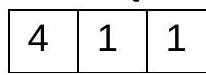
\includegraphics[max width=\textwidth]{2025_02_07_368c3175bd12651af85ag-03}
\end{center}

\section*{Zadania otwarte (niekodowane)}
\section*{Uwagi ogólne:}
\begin{enumerate}
  \item Akceptowane są wszystkie rozwiązania merytorycznie poprawne i spełniające warunki zadania.
  \item Jeżeli zdający popełni błędy rachunkowe, które na żadnym etapie rozwiązania nie upraszczają i nie zmieniają danego zagadnienia, lecz stosuje poprawną metodę i konsekwentnie do popełnionych błędów rachunkowych rozwiązuje zadanie, to może otrzymać co najwyżej ( $n-1$ ) punktów (gdzie $n$ jest maksymalną możliwą do uzyskania liczbą punktów za dane zadanie).
\end{enumerate}

\section*{Zadanie 6. (0-3)}
\begin{center}
\begin{tabular}{|l|l|}
\hline
\multicolumn{2}{|c|}{Wymagania egzaminacyjne 2022} \\
\hline
\multicolumn{1}{|c|}{Wymaganie ogólne} & \multicolumn{1}{c|}{Wymaganie szczegółowe} \\
\hline
V. Rozumowanie i argumentacja. & Zdajacy: \\
 & R2.1) używa wzorów skróconego mnożenia \\
 & na $(a \pm b)^{3}$ oraz $a^{3} \pm b^{3}$. \\
\hline
\end{tabular}
\end{center}

\section*{Zasady oceniania}
\section*{Zdający otrzymuje}
\begin{itemize}
  \item zastosuje wzór na różnicę sześcianów i zapisze nierówność w postaci
\end{itemize}

$$
\begin{aligned}
& (2 x-y)\left(4 x^{2}+2 x y+y^{2}\right)+2 x y(2 x-y) \geq 0 \text { lub } \\
& (2 x-y)\left(4 x^{2}+2 x y+y^{2}\right) \geq-2 x y(2 x-y)
\end{aligned}
$$

ALBO

\begin{itemize}
  \item zastosuje wzór na sześcian różnicy i zapisze nierówność w postaci\\
$(2 x-y)^{3}+8 x y(2 x-y) \geq 0$ lub\\
$(2 x-y)^{3} \geq-8 x y(2 x-y)$,\\
ALBO
  \item przekształci nierówność do postaci\\
$2 x\left(4 x^{2}-y^{2}\right)+y\left(4 x^{2}-y^{2}\right) \geq 0$ lub\\
$2 x\left(4 x^{2}-y^{2}\right) \geq-y\left(4 x^{2}-y^{2}\right)$, lub\\
$4 x^{2}(2 x+y)-y^{2}(2 x+y) \geq 0$, lub\\
$4 x^{2}(2 x+y) \geq y^{2}(2 x+y)$.\\
Zdający otrzymuje\\
gdy przekształci nierówność do postaci $(2 x-y)(2 x+y)^{2} \geq 0$.
\end{itemize}

\section*{Zdajacy otrzymuje}
gdy przeprowadzi pełne rozumowanie - zdający musi spełnić warunek określony w zasadach oceniania za 2 punkty oraz uzasadnić, że $(2 x-y)>0$, powołując się na założenie, oraz zapisać, że kwadrat każdej liczby rzeczywistej jest nieujemny.

\section*{Uwaga:}
Jeśli zdający sprawdza prawdziwość nierówności jedynie dla wybranych wartości $x$ i $y$, to otrzymuje $\mathbf{0}$ punktów za całe rozwiązanie.

\section*{Przykładowe pełne rozwiązania}
Sposób 1. (różnica sześcianów)\\
Przekształcamy równoważnie nierówność $7 x^{3}+4 x^{2} y \geq y^{3}+2 x y^{2}-x^{3}$, korzystając ze wzoru skróconego mnożenia na różnicę sześcianów:

$$
\begin{gathered}
8 x^{3}-y^{3}+4 x^{2} y-2 x y^{2} \geq 0 \\
(2 x-y)\left(4 x^{2}+2 x y+y^{2}\right)+4 x^{2} y-2 x y^{2} \geq 0 \\
(2 x-y)\left(4 x^{2}+2 x y+y^{2}\right)+2 x y(2 x-y) \geq 0 \\
(2 x-y)\left(4 x^{2}+4 x y+y^{2}\right) \geq 0
\end{gathered}
$$

Korzystamy ze wzoru skróconego mnożenia na kwadrat sumy i otrzymujemy

$$
(2 x-y)(2 x+y)^{2} \geq 0
$$

Z założenia $2 x>y$, więc $(2 x-y)>0$.\\
Kwadrat każdej liczby rzeczywistej jest liczba nieujemną, więc $(2 x+y)^{2} \geq 0$.\\
Zatem wyrażenie $(2 x-y)(2 x+y)^{2}$ jest nieujemne jako iloczyn liczby dodatniej i nieujemnej, więc nierówność $(2 x-y)(2 x+y)^{2} \geq 0$ jest prawdziwa. To oznacza, że nierówność $7 x^{3}+4 x^{2} y \geq y^{3}+2 x y^{2}-x^{3}$ jest także prawdziwa.

Sposób 2. (sześcian różnicy)\\
Przekształcamy nierówność $7 x^{3}+4 x^{2} y \geq y^{3}+2 x y^{2}-x^{3}$ do postaci

$$
8 x^{3}-y^{3}-2 x y^{2}+4 x^{2} y \geq 0
$$

Ponieważ $(2 x-y)^{3}=8 x^{3}-y^{3}-12 x^{2} y+6 x y^{2}$, więc otrzymujemy

$$
\begin{gathered}
8 x^{3}-y^{3}-12 x^{2} y+6 x y^{2}+16 x^{2} y-8 x y^{2} \geq 0 \\
(2 x-y)^{3}+16 x^{2} y-8 x y^{2} \geq 0 \\
(2 x-y)^{3}+8 x y(2 x-y) \geq 0 \\
(2 x-y)\left[(2 x-y)^{2}+8 x y\right] \geq 0 \\
(2 x-y)\left(4 x^{2}-4 x y+y^{2}+8 x y\right) \geq 0 \\
(2 x-y)(2 x+y)^{2} \geq 0
\end{gathered}
$$

Z założenia $2 x>y$, więc $(2 x-y)>0$.\\
Kwadrat każdej liczby rzeczywistej jest liczba nieujemną, więc $(2 x+y)^{2} \geq 0$.\\
Zatem wyrażenie $(2 x-y)(2 x+y)^{2}$ jest nieujemne jako iloczyn liczby dodatniej i nieujemnej, więc nierówność $(2 x-y)(2 x+y)^{2} \geq 0$ jest prawdziwa. To oznacza, że nierówność $7 x^{3}+4 x^{2} y \geq y^{3}+2 x y^{2}-x^{3}$ jest także prawdziwa.

Sposób 3. (różnica kwadratów)\\
Przekształcamy równoważnie nierówność $7 x^{3}+4 x^{2} y \geq y^{3}+2 x y^{2}-x^{3}$, korzystając ze wzoru skróconego mnożenia na różnicę kwadratów:

$$
\begin{gathered}
8 x^{3}-2 x y^{2}+4 x^{2} y-y^{3} \geq 0 \\
2 x\left(4 x^{2}-y^{2}\right)+y\left(4 x^{2}-y^{2}\right) \geq 0 \\
(2 x+y)\left(4 x^{2}-y^{2}\right) \geq 0 \\
(2 x+y)(2 x+y)(2 x-y) \geq 0 \\
(2 x-y)(2 x+y)^{2} \geq 0
\end{gathered}
$$

Z założenia $2 x>y$, więc $(2 x-y)>0$.\\
Kwadrat każdej liczby rzeczywistej jest liczba nieujemną, więc $(2 x+y)^{2} \geq 0$.\\
Zatem wyrażenie $(2 x-y)(2 x+y)^{2}$ jest nieujemne jako iloczyn liczby dodatniej i nieujemnej, więc nierówność $(2 x-y)(2 x+y)^{2} \geq 0$ jest prawdziwa. To oznacza, że nierówność $7 x^{3}+4 x^{2} y \geq y^{3}+2 x y^{2}-x^{3}$ jest także prawdziwa.

Zadanie 7. (0-3)

\begin{center}
\begin{tabular}{|l|l|}
\hline
\multicolumn{2}{|c|}{Wymagania egzaminacyjne 2022} \\
\hline
\multicolumn{1}{|c|}{Wymaganie ogólne} & \multicolumn{1}{|c|}{Wymaganie szczegółowe} \\
\hline
IV. Użycie i tworzenie strategii. & \begin{tabular}{l}
Zdający: \\
 \\
 \\
 \\
 \\
 \\
 \\
 \\
R3.8) rozwiązuje równania [...] z wartością \\
bezwzględną [..]. \\
\hline
\end{tabular} \\
\hline
\end{tabular}
\end{center}

\section*{Zasady oceniania}
\section*{Zdający otrzymuje 1 pkt gdy:}
\begin{itemize}
  \item zapisze przedziaty $(-\infty, 3)$ oraz $\langle 3,+\infty)$ i co najmniej w jednym z nich zapisze poprawną postać równania bez użycia symbolu wartości bezwzględnej\\
ALBO
  \item zapisze alternatywę równań $x-3=2 x+11$ lub $x-3=-2 x-11$ i rozwiąże oba otrzymane równania: $x=-14$ lub $x=-\frac{8}{3}$,\\
ALBO
  \item zapisze równanie $(x-3)^{2}=(2 x+11)^{2}$ i rozwiąże je: $x=-14$ lub $x=-\frac{8}{3}$, ALBO
  \item zapisze alternatywę równań $x-3=2 x+11$ lub $x-3=-2 x-11$ i zapisze założenie $2 x+11 \geq 0$,\\
ALBO
  \item narysuje w jednym układzie współrzędnych wykresy funkcji $f$ i $g$ określonych wzorami $f(x)=|x-3|$ oraz $g(x)=2 x+11$.
\end{itemize}

Zdający otrzymuje 2 pkt\\
gdy:

\begin{itemize}
  \item w każdym z przedziałów $(-\infty, 3)$ oraz $\langle 3,+\infty$ ) zapisze poprawną postać równania $|x-3|=2 x+11$ bez użycia symbolu wartości bezwzględnej i w jednym $z$ tych przedziałów rozwiąże równanie\\
ALBO
  \item rozwiąże alternatywę równań $x-3=2 x+11$ lub $x-3=-2 x-11$ i sprawdzi rachunkowo, czy otrzymane liczby są rozwiązaniami równania $|x-3|=2 x+11$, ale w trakcie rozwiązania popełni błędy rachunkowe,\\
ALBO
  \item zapisze alternatywę równań $x-3=2 x+11$ lub $x-3=-2 x-11$ i założenie $2 x+11 \geq 0$ oraz rozwiąże oba równania: $x=-14$ lub $x=-\frac{8}{3}$,\\
ALBO
  \item zapisze odciętą punktu przecięcia wykresów funkcji $f$ i $g: x=-\frac{8}{3}$.
\end{itemize}

\section*{Zdający otrzymuje}
gdy zastosuje poprawną metodę rozwiązania równania i otrzyma prawidłowy wynik: $x=-\frac{8}{3}$, a w przypadku metody graficznej sprawdzi rachunkowo, że liczba $\left(-\frac{8}{3}\right)$ jest rozwiązaniem równania.

\section*{Uwagi:}
\begin{enumerate}
  \item Jeśli zdający opuści symbol wartości bezwzględnej, nie uwzględniając w żaden sposób przedziału, w którym odpowiednie wyrażenie jest dodatnie/ujemne, i w rezultacie zapisze jedynie alternatywe $x-3=2 x+11$ lub $x-3=-2 x-11$ i na tym poprzestanie, to otrzymuje 0 punktów.
  \item Jeśli zdający rozwiązuje równanie w przedziałach $(-\infty, 3)$ oraz $(3,+\infty)$ i nie rozważa przypadku $x=3$, to może otrzymać co najwyżej 2 punkty za całe rozwiązanie.
  \item Jeśli zdający rozwiązuje równanie w przedziałach $(-\infty, 0)$ oraz $\langle 0,+\infty)$, to otrzymuje 0 punktów za całe rozwiązanie.
  \item Jeśli zdający przedstawia dwa rozwiązania, z których jedno jest w pełni poprawne, a drugie niekompletne/błędne, to może otrzymać co najwyżej 2 punkty za całe rozwiązanie.
\end{enumerate}

\section*{Przykładowe pełne rozwiązania}
\section*{Sposób 1.}
Równanie zapisujemy w każdym z przedziałów ( $-\infty, 3$ ), $\langle 3,+\infty$ ) bez użycia symbolu wartości bezwzględnej.

Gdy $x \in(-\infty, 3)$, to równanie ma postać $3-x=2 x+11$.\\
Równanie $3-x=2 x+11$ ma jedno rozwiązanie $x=-\frac{8}{3}$. Jest to liczba należąca do przedziału $(-\infty, 3)$, więc jest to jedno $z$ rozwiązań równania $|x-3|=2 x+11$.

Gdy $x \in\langle 3,+\infty)$, to równanie ma postać $x-3=2 x+11$.\\
Równanie $x-3=2 x+11$ ma również jedno rozwiązanie $x=-14$. Ta liczba nie należy jednak do przedziału $\langle 3,+\infty$ ), więc nie jest rozwiązaniem równania $| x-3 \mid=2 x+11$.\\
W rezultacie równanie $|x-3|=2 x+11$ ma jedno rozwiązanie: $x=-\frac{8}{3}$.

\section*{Sposób 2.}
Jeżeli istnieją rozwiązania równania $|x-3|=2 x+11$, to są one rozwiązaniami alternatywy równań

$$
x-3=2 x+11 \quad \text { lub } \quad x-3=-2 x-11
$$

Stąd otrzymujemy $x=-14$ lub $x=-\frac{8}{3}$.\\
Sprawdzamy, która z tych liczb jest rozwiązaniem równania $|x-3|=2 x+11$.\\
Gdy $x=-14$, to lewa strona równania jest równa $|-14-3|=17$, natomiast prawa strona jest równa $2 \cdot(-14)+11=-17$. Zatem liczba $(-14)$ nie jest rozwiązaniem równania.

Gdy $x=-\frac{8}{3}$, to lewa strona równania jest równa $\left|-\frac{8}{3}-3\right|=\frac{17}{3}$, natomiast prawa strona jest równa $2 \cdot\left(-\frac{8}{3}\right)+11=\frac{17}{3}$. Zatem liczba $\left(-\frac{8}{3}\right)$ jest rozwiązaniem równania.\\
W rezultacie równanie ma jedno rozwiązanie: $x=-\frac{8}{3}$.\\
Sposób 3.\\
Gdy $2 x+11<0$, czyli $x<-\frac{11}{2}$, to równanie $|x-3|=2 x+11$ jest sprzeczne, gdyż lewa jego strona jest nieujemna, a prawa ujemna.\\
Gdy $2 x+11 \geq 0$, czyli $x \geq-\frac{11}{2}$, to równanie $|x-3|=2 x+11$ jest równoważne alternatywie równań

$$
x-3=2 x+11 \quad \text { lub } \quad x-3=-2 x-11
$$

Stąd otrzymujemy $x=-14$ lub $x=-\frac{8}{3}$.\\
Tylko druga z tych liczb jest nie mniejsza od $\left(-\frac{11}{2}\right)$. Zatem równanie $|x-3|=2 x+11$ ma tylko jedno rozwiązanie: $x=-\frac{8}{3}$.

Zadanie 8. (0-3)

\begin{center}
\begin{tabular}{|c|l|}
\hline
\multicolumn{2}{|c|}{Wymagania egzaminacyjne 2022} \\
\hline
\multicolumn{1}{|c|}{Wymaganie ogólne} & \multicolumn{1}{c|}{Wymaganie szczegółowe} \\
\hline
V. Rozumowanie i argumentacja. & Zdający: \\
 & R7.4) znajduje związki miarowe w figurach \\
 & płaskich z zastosowaniem twierdzenia \\
sinusów i twierdzenia cosinusów. &  \\
\hline
\end{tabular}
\end{center}

\section*{Zasady oceniania}
\section*{Zdajacy otrzymuje}
gdy spełni jeden z poniższych warunków:

\begin{enumerate}
  \item zapisze związek między długością jednej z podstaw trapezu a promieniem $R_{2}$ okręgu opisanego na trójkącie CPD (lub promieniem $R_{1}$ okręgu opisanego na trójkącie $A P B)$, np. $\frac{|C D|}{R_{2}}=\frac{|C D|+2}{R_{2}+3}, \frac{|A B|-2}{R_{2}}=\frac{|A B|}{R_{2}+3}, \frac{|A B|}{R_{1}}=\frac{|A B|-2}{R_{1}-3}$
  \item zapisze związki między długościami podstaw trapezu, promieniami okręgów opisanych na trójkątach $A B P$ i $C D P$ oraz związek między długościami podstaw trapezu i promieniami okręgów, np. $|A B|=|C D|+2$ i $R_{1}=R_{2}+3$ i $\frac{|A B|}{R_{1}}=\frac{|C D|}{R_{2}}$,
  \item zapisze związki: $\frac{|A B|}{\sin \alpha}=2 R_{1}, \frac{|C D|}{\sin \alpha}=2 R_{2},|C D|+2=|A B|, R_{1}=R_{2}+3$,
  \item zapisze równanie $z$ dwiema niewiadomymi - długością jednej $z$ podstaw trapezu i sinusem kąta $\alpha, \mathrm{np} . \frac{|C D|}{\sin \alpha}=\frac{|C D|+2}{\sin \alpha}-6$,
  \item zapisze warunek $\cos \alpha=\frac{4 \sqrt{2}}{6}$ jako warunek równoważny tezie.\\
$\qquad$\\
Zdający otrzymuje 2 pkt gdy:
\end{enumerate}

\begin{itemize}
  \item gdy spełni jeden z warunków 1)-4) zapisanych w zasadach oceniania za 1 punkt oraz obliczy $\sin \alpha: \sin \alpha=\frac{1}{3}$\\
ALBO
  \item zastosuje twierdzenie cosinusów do trójkąta $A S_{1} B$ i obliczy wartość cosinusa kąta środkowego opartego na tym samym łuku, co kąt $A P B$ : $\cos 2 \alpha=\frac{7}{9}$ (sposób 4.).
\end{itemize}

Zdający otrzymuje 3 pkt gdy przeprowadzi pełne rozumowanie.

\section*{Uwagi:}
\begin{enumerate}
  \item Jeśli zdający wprowadzi do rozwiązania dodatkowe założenia, nie wynikające z treści zadania, i korzysta z tych założeń, to za całe rozwiązanie otrzymuje $\mathbf{0}$ punktów, o ile nie nabył praw do innej punktacji.
  \item Jeśli zdający $w$ wyniku popełnionego błędu otrzyma równość $\sin \alpha=\frac{1}{3}$, to może otrzymać co najwyżej 1 punkt za całe rozwiązanie.
\end{enumerate}

\section*{Przykładowe pełne rozwiązania}
Sposób 1. (podobieństwo trójkątów)\\
Oznaczmy przez $R_{2}$ promień okręgu opisanego na trójkącie $C P D$, a przez $\alpha$ - miarę kąta ostrego CPD.\\
Ponieważ odcinki $A B$ i $C D$ są równoległe, więc $|\Varangle P C D|=|\Varangle P A B|$ i $|\Varangle A B P|=|\Varangle P D C|$ (kąty naprzemianległe) oraz $|\Varangle C P D|=|\Varangle A P B|$ (kąty wierzchołkowe). Zatem trójkąty CPD i $A P B$ są podobne (na mocy cechy kkk). Stąd wynika, że

$$
\frac{R_{2}+3}{|A B|}=\frac{R_{2}}{|C D|}
$$

i wobec $|A B|=|C D|+2$ otrzymujemy dalej

$$
\begin{gathered}
\frac{R_{2}+3}{|C D|+2}=\frac{R_{2}}{|C D|} \\
2 R_{2}=3 \cdot|C D| \\
|C D|=\frac{2}{3} R_{2}
\end{gathered}
$$

Do trójkąta CPD stosujemy twierdzenie sinusów i otrzymujemy

$$
\frac{|C D|}{\sin \alpha}=2 R_{2}
$$

co w połączeniu ze związkiem $|C D|=\frac{2}{3} R_{2}$ prowadzi do równania

$$
\sin \alpha=\frac{1}{3}
$$

Korzystamy z tożsamości trygonometrycznej $\sin ^{2} \alpha+\cos ^{2} \alpha=1$ i, uwzględniając, że $\alpha<90^{\circ}$, otrzymujemy

$$
\begin{gathered}
\left(\frac{1}{3}\right)^{2}+\cos ^{2} \alpha=1 \\
\cos \alpha=\frac{2 \sqrt{2}}{3}
\end{gathered}
$$

Do trójkąta CPD stosujemy twierdzenie cosinusów, korzystamy ze związku $\cos \alpha=\frac{2 \sqrt{2}}{3}$ i otrzymujemy

$$
\begin{gathered}
|C D|^{2}=|D P|^{2}+|C P|^{2}-2 \cdot|D P| \cdot|C P| \cdot \cos \alpha \\
|C D|^{2}=|D P|^{2}+|C P|^{2}-2 \cdot|D P| \cdot|C P| \cdot \frac{2 \sqrt{2}}{3} \\
\frac{4 \sqrt{2}}{3} \cdot|D P| \cdot|C P|=|D P|^{2}+|C P|^{2}-|C D|^{2}
\end{gathered}
$$

To należało pokazać.

Sposób 2. (twierdzenie sinusów)\\
Oznaczmy przez $R_{2}$ promień okręgu opisanego na trójkącie $C P D$, a przez $\alpha$ - miarę kąta ostrego CPD.\\
Ponieważ kąty ostre $C P D$ i $A P B$ są wierzchołkowe, to $|\Varangle C P D|=|\Varangle A P B|=\alpha$.\\
Do trójkątów $A P B$ i $C P D$ stosujemy twierdzenie sinusów i otrzymujemy

$$
\frac{|A B|}{\sin \alpha}=2\left(R_{2}+3\right) \quad \text { oraz } \quad \frac{|C D|}{\sin \alpha}=2 R_{2}
$$

Stąd $\frac{|A B|}{2\left(R_{2}+3\right)}=\frac{|C D|}{2 R_{2}}$, a ponieważ z założenia $|A B|=|C D|+2$, więc $\frac{|C D|+2}{2\left(R_{2}+3\right)}=\frac{|C D|}{2 R_{2}}$ i w rezultacie

$$
|C D|=\frac{2}{3} R_{2}
$$

Ze związków $|C D|=\frac{2}{3} R_{2}$ i $\frac{|C D|}{\sin \alpha}=2 R_{2}$ otrzymujemy

$$
\sin \alpha=\frac{1}{3}
$$

Korzystamy z tożsamości trygonometrycznej $\sin ^{2} \alpha+\cos ^{2} \alpha=1$ i, uwzględniając, że $\alpha<90^{\circ}$, otrzymujemy

$$
\begin{gathered}
\left(\frac{1}{3}\right)^{2}+\cos ^{2} \alpha=1 \\
\cos \alpha=\frac{2 \sqrt{2}}{3}
\end{gathered}
$$

Do trójkąta CPD stosujemy twierdzenie cosinusów, korzystamy ze związku $\cos \alpha=\frac{2 \sqrt{2}}{3}$ i otrzymujemy

$$
\begin{aligned}
& |C D|^{2}=|D P|^{2}+|C P|^{2}-2 \cdot|D P| \cdot|C P| \cdot \cos \alpha \\
& |C D|^{2}=|D P|^{2}+|C P|^{2}-2 \cdot|D P| \cdot|C P| \cdot \frac{2 \sqrt{2}}{3}
\end{aligned}
$$

$$
\frac{4 \sqrt{2}}{3} \cdot|D P| \cdot|C P|=|D P|^{2}+|C P|^{2}-|C D|^{2}
$$

To należało pokazać.

\section*{Sposób 3.}
Oznaczmy przez $R_{2}$ promień okręgu opisanego na trójkącie $C P D$, a przez $\alpha$ - miarę kąta ostrego CPD.\\
Ponieważ kąty ostre $C P D$ i $A P B$ są wierzchołkowe, to $|\Varangle C P D|=|\Varangle A P B|=\alpha$.\\
Do trójkątów $A P B$ i $C P D$ stosujemy twierdzenie sinusów i otrzymujemy

$$
\frac{|A B|}{\sin \alpha}=2\left(R_{2}+3\right) \quad \text { oraz } \quad \frac{|C D|}{\sin \alpha}=2 R_{2}
$$

Łącząc obie te zależności i korzystając z założenia $|A B|=|C D|+2$, otrzymujemy

$$
\begin{gathered}
\frac{|A B|}{\sin \alpha}=\frac{|C D|}{\sin \alpha}+6 \\
\frac{|C D|+2}{\sin \alpha}=\frac{|C D|}{\sin \alpha}+6 \\
\frac{|C D|}{\sin \alpha}+\frac{2}{\sin \alpha}=\frac{|C D|}{\sin \alpha}+6 \\
\sin \alpha=\frac{1}{3}
\end{gathered}
$$

Korzystamy z tożsamości trygonometrycznej $\sin ^{2} \alpha+\cos ^{2} \alpha=1$ i, uwzględniając, że $\alpha<90^{\circ}$, otrzymujemy

$$
\begin{gathered}
\left(\frac{1}{3}\right)^{2}+\cos ^{2} \alpha=1 \\
\cos \alpha=\frac{2 \sqrt{2}}{3}
\end{gathered}
$$

Do trójkąta CPD stosujemy twierdzenie cosinusów, korzystamy ze związku $\cos \alpha=\frac{2 \sqrt{2}}{3}$ i otrzymujemy

$$
\begin{gathered}
|C D|^{2}=|D P|^{2}+|C P|^{2}-2 \cdot|D P| \cdot|C P| \cdot \cos \alpha \\
|C D|^{2}=|D P|^{2}+|C P|^{2}-2 \cdot|D P| \cdot|C P| \cdot \frac{2 \sqrt{2}}{3} \\
\frac{4 \sqrt{2}}{3} \cdot|D P| \cdot|C P|=|D P|^{2}+|C P|^{2}-|C D|^{2}
\end{gathered}
$$

To należało pokazać.

\section*{Sposób 4. (kąt wpisany - kąt środkowy)}
Niech $o_{1}$ będzie okręgiem o środku $S_{1}$ i promieniu $R_{1}$ opisanym na trójkącie $A P B$.\\
Oznaczmy przez $\alpha$ miarę kąta ostrego $A P B$.\\
Ponieważ odcinki $A B$ i $C D$ są równoległe, więc $|\Varangle P C D|=|\Varangle P A B|$ i $|\Varangle A B P|=|\Varangle P D C|$\\
(kąty naprzemianległe) oraz $|\Varangle C P D|=|\Varangle A P B|$ (kąty wierzchołkowe).\\
Na mocy cechy kkk trójkąty $C P D$ i $A P B$ są podobne.\\
Niech $x=|A B|$. Wtedy $|C D|=x-2$. Z podobieństwa trójkątów $C P D$ i $A P B$ wynika równość

$$
\frac{x-2}{x}=\frac{R_{1}-3}{R_{1}}
$$

skąd otrzymujemy $R_{1}=\frac{3}{2} x$.\\
Zauważmy, że $2 \alpha$ jest miarą kąta środkowego, opartego na tym samym łuku okręgu $o_{1}$, co kąt $A P B$. Korzystamy z twierdzenia cosinusów zastosowanego do trójkąta $A S_{1} B$ i otrzymujemy kolejno

$$
\begin{gathered}
x^{2}=2 R_{1}^{2} \cdot(1-\cos 2 \alpha) \\
x^{2}=2 \cdot\left(\frac{3}{2} x\right)^{2} \cdot(1-\cos 2 \alpha)
\end{gathered}
$$

skąd po obustronnym podzieleniu przez $x^{2}$ otrzymujemy równość

$$
1=\frac{9}{2} \cdot(1-\cos 2 \alpha)
$$

Zatem $\cos 2 \alpha=\frac{7}{9}$. Jest ona równoważna równości $2 \cos ^{2} \alpha-1=\frac{7}{9}$, z której obliczamy $\cos \alpha=\frac{2 \sqrt{2}}{3}$ (ujemną wartość odrzucamy ze względu na to, że kąt o mierze $\alpha$ jest kątem wewnętrznym trójkąta ostrokątnego CPD).\\
Do trójkąta $C P D$ stosujemy twierdzenie cosinusów, korzystamy ze związku $\cos \alpha=\frac{2 \sqrt{2}}{3}$ i otrzymujemy

$$
\begin{gathered}
|C D|^{2}=|D P|^{2}+|C P|^{2}-2 \cdot|D P| \cdot|C P| \cdot \cos \alpha \\
|C D|^{2}=|D P|^{2}+|C P|^{2}-2 \cdot|D P| \cdot|C P| \cdot \frac{2 \sqrt{2}}{3} \\
\frac{4 \sqrt{2}}{3} \cdot|D P| \cdot|C P|=|D P|^{2}+|C P|^{2}-|C D|^{2}
\end{gathered}
$$

To należało pokazać.

Zadanie 9. (0-4)

\begin{center}
\begin{tabular}{|l|l|}
\hline
\multicolumn{2}{|c|}{Wymagania egzaminacyjne 2022} \\
\hline
\multicolumn{1}{|c|}{Wymaganie ogólne} & \multicolumn{1}{|c|}{Wymagania szczegółowe} \\
\hline
IV. Użycie i tworzenie strategii. & Zdający: \\
 & R3.4) stosuje twierdzenie o reszcie \\
 & z dzielenia wielomianu przez dwumian $x-a ;$ \\
 & R3.6) rozwiązuje łatwe nierówności \\
 & wielomianowe. \\
\hline
\end{tabular}
\end{center}

\section*{Zasady oceniania}
\section*{Zdający otrzymuje \\
 1 pkt}
gdy:

\begin{itemize}
  \item zapisze równanie $z$ niewiadomą $m$ wynikające $z$ warunków zadania:
\end{itemize}

$$
4 \cdot(-2)^{3}-6 \cdot(-2)^{2}-(5 m+1) \cdot(-2)-2 m=-30
$$

\section*{ALBO}
\begin{itemize}
  \item wyznaczy resztę z dzielenia wielomianu $W$ przez dwumian $(x+2)$ i zapisze równanie $-2 m+2(5 m-27)=-30$.\\
Zdający otrzymuje
\end{itemize}

gdy obliczy $m$ : $m=3$.

\section*{Zdajacy otrzymuje}
gdy obliczy/poda wszystkie pierwiastki wielomianu $W(x)=4 x^{3}-6 x^{2}-16 x-6$ :\\
$x_{1}=-1, x_{2}=-\frac{1}{2}, x_{3}=3$.

\section*{Zdający otrzymuje}
gdy rozwiąże nierówność $W(x) \geq 0: x \in\left\langle-1,-\frac{1}{2}\right\rangle \cup\langle 3,+\infty\rangle$.

\section*{Uwagi:}
\begin{enumerate}
  \item Jeżeli zdający poprawnie interpretuje warunki zadania $W(-2)=-30$, ale popełnia błędy rachunkowe, zapisując równanie wynikające $z$ tego warunku, to może otrzymać co najwyżej 3 punkty za całe rozwiązanie.
  \item Jeżeli zdający popełnia błąd $w$ interpretacji warunków zadania, zapisując np. $W(2)=-30$, w konsekwencji którego zapisuje błędne równanie wynikające z tego warunku, lecz otrzyma wielomian o trzech różnych pierwiastkach i konsekwentnie doprowadzi rozwiązanie do końca, to otrzymuje 2 punkty za całe rozwiązanie.
  \item Jeżeli zdający w wyniku błędów rachunkowych przekształci wielomian $W$ do postaci, w której otrzymany wielomian ma co najwyżej dwa pierwiastki (jeden dwukrotny i jeden pierwiastek jednokrotny), to za całe rozwiązanie może otrzymać co najwyżej:\\
3 punkty - jeśli uwzględnia krotności pierwiastków,\\
2 punkty - jeśli nie uwzględnia krotności pierwiastków.
\end{enumerate}

\section*{Przykładowe pełne rozwiązanie}
Reszta z dzielenia wielomianu $W$ przez dwumian $x+2$ jest równa ( -30 ), zatem $W(-2)=-30$. Stąd otrzymujemy

$$
4 \cdot(-2)^{3}-6 \cdot(-2)^{2}-(5 m+1)(-2)-2 m=-30
$$

Rozwiązaniem tego równania jest $m=3$.\\
Rozwiązujemy nierówność $4 x^{3}-6 x^{2}-16 x-6 \geq 0$, stosując przekształcenia równoważne, i otrzymujemy kolejno:

$$
\begin{gathered}
4 x^{3}-6 x^{2}-16 x-6 \geq 0 \\
2(x+1)\left(2 x^{2}-5 x-3\right) \geq 0 \\
4(x+1)(x-3)\left(x+\frac{1}{2}\right) \geq 0
\end{gathered}
$$

Szkicujemy wykres wielomianu $W(x)=4(x+1)(x-3)\left(x+\frac{1}{2}\right)$\\
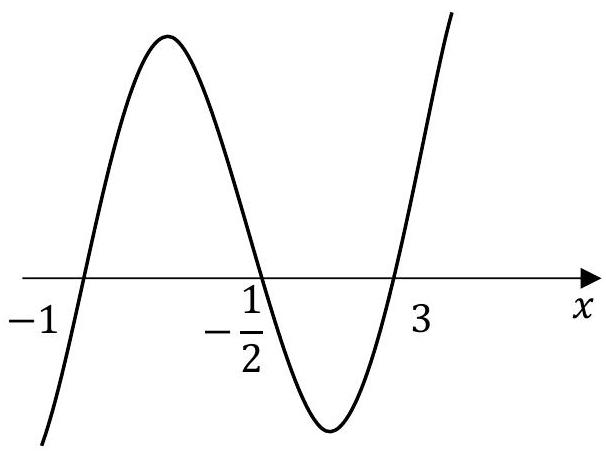
\includegraphics[max width=\textwidth, center]{2025_02_07_368c3175bd12651af85ag-16}\\
i odczytujemy zbiór rozwiązań nierówności $W(x) \geq 0:\left\langle-1,-\frac{1}{2}\right\rangle \cup\langle 3,+\infty)$.

Zadanie 10. (0-4)

\begin{center}
\begin{tabular}{|l|l|}
\hline
\multicolumn{2}{|c|}{Wymagania egzaminacyjne 2022} \\
\hline
\multicolumn{1}{|c|}{Wymaganie ogólne} & \multicolumn{1}{c|}{Wymagania szczegółowe} \\
\hline
III. Modelowanie matematyczne. & Zdający: \\
 & P5.3) stosuje wzór na n-ty wyraz i na \\
 & sumę n początkowych wyrazów ciągu \\
 & arytmetycznego; \\
 & R5.2) rozpoznaje szeregi geometryczne \\
 & zbieżne i oblicza ich sumy. \\
\hline
\end{tabular}
\end{center}

Zasady oceniania dla sposobów 1. i 2.

\section*{Zdający otrzymuje 1 pkt gdy:}
\begin{itemize}
  \item obliczy iloraz $q$ ciągu $\left(a_{n}\right): q=\frac{2}{5}$
\end{itemize}

ALBO

\begin{itemize}
  \item zapisze $b_{1}+3 r=b_{4}$,
\end{itemize}

ALBO

\begin{itemize}
  \item zapisze $S_{25}=\frac{b_{1}+b_{25}}{2} \cdot 25$ lub $S_{25}=\frac{2 b_{1}+24 r}{2} \cdot 25$.
\end{itemize}

Zdający otrzymuje 2 pkt gdy:

\begin{itemize}
  \item zapisze równanie z dwiema niewiadomymi $b_{1}$ i $r$, np. $b_{1}+3 r=108$,
\end{itemize}

$$
1125=\frac{2 b_{1}+24 r}{2} \cdot 25
$$

ALBO

\begin{itemize}
  \item zapisze $S_{25}=\frac{2 b_{1}+24 r}{2} \cdot 25$ oraz $b_{1}+3 r=b_{4}$.
\end{itemize}

Zdający otrzymuje .................................................................................................... 3 pkt\\
gdy zapisze układ dwóch niezależnych równań z dwiema niewiadomymi $b_{1}$ i $r$, np.\\
$b_{1}+3 r=108$ oraz $1125=\frac{2 b_{1}+24 r}{2} \cdot 25$.\\
Zdający otrzymuje 4 pkt\\
gdy obliczy $b_{1}$ : $b_{1}=129$.

\section*{Uwagi:}
\begin{enumerate}
  \item Jeżeli zdający myli własności ciągu arytmetycznego z własnościami ciągu geometrycznego, to otrzymuje 0 punktów za całe rozwiązanie.
  \item Jeśli zdający rozpatruje przypadek $q=0$ i w ostatecznej odpowiedzi nie odrzuca otrzymanej z tego przypadku wartości $b_{1}$, to może otrzymać co najwyżej 3 punkty za całe rozwiązanie.
  \item Jeśli zdający, obliczając iloraz ciągu ( $a_{n}$ ), popełni błąd i otrzyma jedynie wartość ilorazu $q$ spoza przedziału ( $-1,1$ ), to może otrzymać co najwyżej 1 punkt za całe rozwiązanie.
  \item Jeśli zdający, obliczając iloraz ciągu ( $a_{n}$ ), popełni błąd i uzyska wartość ilorazu ze zbioru $(-1,0) \cup(0,1)$, to może otrzymać za całe rozwiązanie co najwyżej:\\
3 punkty - gdy popełni jedynie błąd rachunkowy (lub błąd nieuwagi),\\
2 punkty - gdy popełni błąd rzeczowy.
\end{enumerate}

\section*{Przykładowe pełne rozwiązania}
\section*{Sposób 1.}
Korzystamy z własności ciągu geometrycznego i przekształcamy równanie $a_{22}=\frac{5}{4} a_{23}+\frac{1}{5} a_{21}$ do postaci $a_{21} \cdot q=\frac{5}{4} a_{21} \cdot q^{2}+\frac{1}{5} a_{21}$. Dzieląc obie strony równania przez $a_{21} \neq 0$, otrzymujemy równanie $\frac{5}{4} q^{2}-q+\frac{1}{5}=0$, którego rozwiązaniem jest $q=\frac{2}{5}$.\\
Ponieważ $|q|=\left|\frac{2}{5}\right|<1$, zatem istnieje suma $S$ wszystkich wyrazów ciągu $\left(a_{n}\right)$.\\
Obliczamy sume $S=\frac{675}{1-\frac{2}{5}}=1125$ i $a_{3}=675 \cdot\left(\frac{2}{5}\right)^{2}=108$.\\
Trzeci wyraz ciągu geometrycznego jest równy czwartemu wyrazowi ciągu arytmetycznego, więc $b_{4}=b_{1}+3 r=108$.\\
Suma wszystkich wyrazów nieskończonego ciągu geometrycznego $\left(a_{n}\right)$ jest równa sumie dwudziestu pięciu początkowych wyrazów ciągu arytmetycznego $\left(b_{n}\right)$, zatem

$$
\begin{gathered}
1125=\frac{2 b_{1}+24 r}{2} \cdot 25 \\
45=b_{1}+12 r
\end{gathered}
$$

Z równań $b_{1}+3 r=108$ i $b_{1}+12 r=45$ otrzymujemy $r=-7$.\\
Zatem $b_{1}=108-3 \cdot(-7)=129$.

\section*{Sposób 2.}
Korzystamy z własności ciągu geometrycznego i przekształcamy równanie $a_{22}=\frac{5}{4} a_{23}+\frac{1}{5} a_{21}$ do postaci $a_{2} \cdot q^{20}=\frac{5}{4} a_{3} \cdot q^{20}+\frac{1}{5} a_{1} \cdot q^{20}$. Dzieląc obie strony równania przez $q$ (wszystkie wyrazy ciągu są dodatnie, więc $q \neq 0$ ), otrzymujemy $a_{2}=\frac{5}{4} a_{3}+\frac{1}{5} a_{1}$. Stąd i z własności ciągu geometrycznego otrzymujemy dalej

$$
\left(\frac{5}{4} a_{3}+\frac{1}{5} a_{1}\right)^{2}=675 \cdot a_{3}
$$

$$
\frac{25}{16} a_{3}^{2}-\frac{675}{2} a_{3}+18225=0
$$

Rozwiązaniem równania jest $a_{3}=108$. Stosujemy wzór na $n$-ty wyraz ciągu\\
geometrycznego i zapisujemy $108=675 \cdot q^{2}$, skąd $q=\frac{2}{5}$ lub $q=-\frac{2}{5}$. Ponieważ wszystkie wyrazy ciągu $\left(a_{n}\right)$ są dodatnie, więc $q=\frac{2}{5}$.\\
Stwierdzamy, że $|q|<1$, więc istnieje suma $S$ wszystkich wyrazów ciągu ( $a_{n}$ ). Obliczamy sumę $S=\frac{675}{1-\frac{2}{5}}=1125$.\\
Trzeci wyraz ciągu geometrycznego jest równy czwartemu wyrazowi ciągu arytmetycznego, więc $b_{4}=b_{1}+3 r=108$.\\
Suma wszystkich wyrazów nieskończonego ciągu geometrycznego $\left(a_{n}\right)$ jest równa sumie dwudziestu pięciu początkowych wyrazów ciągu arytmetycznego $\left(b_{n}\right)$, zatem

$$
\begin{gathered}
1125=\frac{2 b_{1}+24 r}{2} \cdot 25 \\
45=b_{1}+12 r
\end{gathered}
$$

Z równań $b_{1}+3 r=108$ i $b_{1}+12 r=45$ otrzymujemy $r=-7$.\\
Zatem $b_{1}=108-3 \cdot(-7)=129$.

\section*{Zadanie 11. (0-4)}
\begin{center}
\begin{tabular}{|l|l|}
\hline
\multicolumn{2}{|c|}{Wymagania egzaminacyjne 2022} \\
\hline
\multicolumn{1}{|c|}{Wymaganie ogólne} & \multicolumn{1}{c|}{Wymagania szczegółowe} \\
\hline
IV. Użycie i tworzenie strategii. & Zdający: \\
 & R6.5) stosuje wzory na sinus i cosinus sumy \\
 & i różnicy kątów, sumę i różnicę sinusów \\
 & i cosinusów kąów; \\
 & R6.6) rozwiązuje równania \\
 & trygonometryczne [...]. \\
\hline
\end{tabular}
\end{center}

\section*{Zasady oceniania}
\section*{Zdający otrzymuje}
gdy:

\begin{itemize}
  \item przekształci równoważnie równanie $\sin x+\sin 2 x+\sin 3 x=0$, stosując wzór na sumę sinusów lub sinus sumy, lub sinus różnicy, lub sinus podwojonego kąta, lub sinus potrojonego kąta, np.:\\
$2 \sin 2 x \cos (-x)+\sin 2 x=0$\\
lub\\
$2 \sin (1,5 x) \cos (-0,5 x)+\sin 3 x=0$,\\
lub\\
$\sin x+2 \sin (2,5 x) \cos (-0,5 x)=0$,\\
lub\\
$\sin x+\sin 2 x+\sin x \cos 2 x+\cos x \sin 2 x=0$,\\
lub\\
$\sin 2 x \cos x-\cos 2 x \sin x+\sin 2 x+\sin x \cos 2 x+\cos x \sin 2 x=0$,\\
lub\\
$\sin x+\sin 2 x+2 \sin (1,5 x) \cos (1,5 x)=0$,\\
lub\\
$\sin x+\sin 2 x+3 \sin x-4 \sin ^{3} x=0$,\\
ALBO
  \item poda dwie spośród liczb: $0, \frac{\pi}{2}, \pi$, i zapisze, że podane liczby spełniają równanie.
\end{itemize}

\section*{Zdający otrzymuje}
gdy przekształci równanie $\sin x+\sin 2 x+\sin 3 x=0$ do postaci alternatywy równań trygonometrycznych, np.:\\
$\sin 2 x=0$ lub $2 \cos x+1=0$,\\
$\sin (1,5 x)=0$ lub $\cos (-0,5 x)+\cos (1,5 x)=0$,\\
$\cos (0,5 x)=0$ lub $\sin (0,5 x)+\sin (2,5 x)=0$,\\
$\sin x=0$ lub $4 \cos ^{2} x+2 \cos x=0$.

\section*{Zdający otrzymuje \\
 gdy:}
\begin{itemize}
  \item przekształci równanie $\sin x+\sin 2 x+\sin 3 x=0$ do postaci alternatywy równań trygonometrycznych i rozwiąże każde z tych równań w zbiorze liczb rzeczywistych ALBO
  \item przekształci równanie $\sin x+\sin 2 x+\sin 3 x=0$ do postaci alternatywy równań trygonometrycznych i rozwiąże jedno z tych równań w przedziale $\langle 0, \pi\rangle$.
\end{itemize}

\section*{Zdajacy otrzymuje}
gdy zastosuje poprawną metodę rozwiązania równania $\sin x+\sin 2 x+\sin 3 x=0$\\
i otrzyma poprawny zbiór rozwiązań w przedziale $\langle 0, \pi\rangle$ : $\left\{0, \frac{\pi}{2}, \frac{2 \pi}{3}, \pi\right\}$.

\section*{Uwagi:}
\begin{enumerate}
  \item Jeśli zdający popełnia jednokrotnie błąd polegający na:
\end{enumerate}

\begin{itemize}
  \item niepoprawnym zastosowaniu wzorów trygonometrycznych na: sinus sumy/różnicy lub sumę/różnicę sinusów, lub sinus podwojonego/potrojonego kąta\\
ALBO
  \item błędnym zastosowaniu nieparzystości/parzystości funkcji trygonometrycznej\\
i konsekwentnie rozwiąże zadanie do końca oraz otrzyma co najmniej trzy rozwiązania z przedziału $\langle 0, \pi\rangle$, to może otrzymać co najwyżej 2 punkty za całe rozwiązanie, o ile nie nabył praw do innej punktacji.
\end{itemize}

\begin{enumerate}
  \setcounter{enumi}{1}
  \item Jeśli zdający zastępuje $\cos x$ przez $\sqrt{1-\sin ^{2} x}$ i konsekwentnie rozwiąże zadanie do końca, otrzymując co najmniej trzy rozwiązania z przedziału $\langle 0, \pi\rangle$, to może otrzymać co najwyżej 2 punkty za całe rozwiązanie.
  \item Jeśli zdający dzieli obie strony równania przez wyrażenie $a(x)$ zawierające niewiadomą $x$ i nie rozważa przypadku $a(x)=0$, ale konsekwentnie rozwiąże zadanie do końca i otrzyma co najmniej trzy rozwiązania z przedziału $\langle 0, \pi\rangle$, to może otrzymać co najwyżej 2 punkty za całe rozwiązanie.
\end{enumerate}

\section*{Przykładowe pełne rozwiązania}
Sposób 1. (suma sinusów)\\
Przekształcamy równanie w sposób równoważny:

$$
\begin{aligned}
& \sin x+\sin 3 x+\sin 2 x=0 \\
& 2 \sin 2 x \cos (-x)+\sin 2 x=0 \\
& \sin 2 x(2 \cos x+1)=0 \\
& \quad \sin 2 x=0 \text { lub } \cos x=-\frac{1}{2}
\end{aligned}
$$

Stąd $2 x=k \pi$ lub $x=\frac{2 \pi}{3}+2 k \pi$ lub $x=\frac{4 \pi}{3}+2 k \pi$, gdzie $k$ jest liczbą całkowita. Zatem $x=k \cdot \frac{\pi}{2}$ lub $x=\frac{2 \pi}{3}+2 k \pi$ lub $x=\frac{4 \pi}{3}+2 k \pi$, gdzie $k$ jest liczbą całkowita. Rozwiązaniami równania $\sin x+\sin 2 x+\sin 3 x=0$ w przedziale $\langle 0, \pi\rangle$ są liczby: $0, \frac{\pi}{2}$, $\frac{2 \pi}{3}, \pi$.

\section*{Inne przykładowe realizacje.}
1.

Przekształcamy równanie w sposób równoważny:

$$
\begin{gathered}
\sin x+\sin 2 x+\sin 3 x=0 \\
2 \sin (1,5 x) \cos (-0,5 x)+\sin 3 x=0 \\
2 \sin (1,5 x) \cos (-0,5 x)+2 \sin (1,5 x) \cos (1,5 x)=0 \\
2 \sin (1,5 x)(\cos (-0,5 x)+\cos (1,5 x))=0 \\
2 \sin (1,5 x)=0 \text { lub } \cos (-0,5 x)+\cos (1,5 x)=0 \\
2 \sin (1,5 x)=0 \text { lub } 2 \cos (0,5 x) \cos (-x)=0
\end{gathered}
$$

Stąd $1,5 x=k \pi$ lub $0,5 x=\frac{\pi}{2}+k \pi$ lub $x=\frac{\pi}{2}+k \pi$, gdzie $k$ jest liczbą całkowita. Zatem $x=\frac{2 \pi}{3} \cdot k$ lub $x=\pi+2 k \pi$ lub $x=\frac{\pi}{2}+k \pi$, gdzie $k$ jest liczbą całkowitą. Rozwiązaniami równania $\sin x+\sin 2 x+\sin 3 x=0$ w przedziale $\langle 0, \pi\rangle$ są liczby: $0, \frac{\pi}{2}$, $\frac{2 \pi}{3}, \pi$.

\section*{2)}
Przekształcamy równanie w sposób równoważny:

$$
\begin{gathered}
\sin x+\sin 2 x+\sin 3 x=0 \\
\sin x+2 \sin (2,5 x) \cos (-0,5 x)=0 \\
2 \sin (0,5 x) \cos (0,5 x)+2 \sin (2,5 x) \cos (0,5 x)=0 \\
2 \cos (0,5 x)(\sin (0,5 x)+\sin (2,5 x))=0 \\
2 \cos (0,5 x)=0 \text { lub } \sin (0,5 x)+\sin (2,5 x)=0 \\
2 \cos (0,5 x)=0 \text { lub } 2 \sin (1,5 x) \cos (-x)=0
\end{gathered}
$$

Stąd $0,5 x=\frac{\pi}{2}+k \pi$ lub $1,5 x=k \pi$ lub $x=\frac{\pi}{2}+k \pi$, gdzie $k$ jest liczbą całkowita.\\
Zatem $x=\pi+2 k \pi$ lub $x=\frac{2 \pi}{3} \cdot k$ lub $x=\frac{\pi}{2}+k \pi$, gdzie $k$ jest liczbą całkowitą.

Rozwiązaniami równania $\sin x+\sin 2 x+\sin 3 x=0 \mathrm{w}$ przedziale $\langle 0, \pi\rangle$ są liczby: $0, \frac{\pi}{2}$, $\frac{2 \pi}{3}, \pi$.

Sposób 2. (sinus sumy)\\
Przekształcamy równanie w sposób równoważny:

$$
\begin{gathered}
\sin x+\sin 2 x+\sin 3 x=0 \\
\sin x+\sin 2 x+\sin (x+2 x)=0 \\
\sin x+\sin 2 x+\sin x \cos 2 x+\cos x \sin 2 x=0 \\
\sin x\left(1+2 \cos x+\cos 2 x+2 \cos ^{2} x\right)=0 \\
\sin x\left(1+2 \cos x+2 \cos ^{2} x-1+2 \cos ^{2} x\right)=0 \\
\sin x=0 \text { lub } 4 \cos ^{2} x+2 \cos x=0 \\
\sin x=0 \text { lub } \cos x=0 \text { lub } 2 \cos x+1=0
\end{gathered}
$$

Stąd $x=k \pi$ lub $x=\frac{\pi}{2}+k \pi$ lub $x=\frac{2 \pi}{3}+2 k \pi$ lub $x=\frac{4 \pi}{3}+2 k \pi$, gdzie $k$ jest liczba całkowitą.\\
Rozwiązaniami równania $\sin x+\sin 2 x+\sin 3 x=0$ w przedziale $\langle 0, \pi\rangle$ są liczby: $0, \frac{\pi}{2}$, $\frac{2 \pi}{3}, \pi$.

Sposób 3. (sinus różnicy)\\
Przekształcamy równanie w sposób równoważny:

$$
\begin{gathered}
\sin x+\sin 2 x+\sin 3 x=0 \\
\sin (2 x-x)+\sin 2 x+\sin (x+2 x)=0 \\
\sin 2 x \cos x-\cos 2 x \sin x+\sin 2 x+\sin x \cos 2 x+\cos x \sin 2 x=0 \\
2 \sin 2 x \cos x+\sin 2 x=0 \\
\sin 2 x(2 \cos x+1)=0
\end{gathered}
$$

I dalej jak w sposobie 1.

\section*{Zadanie 12. (0-5)}
\begin{center}
\begin{tabular}{|l|l|}
\hline
\multicolumn{2}{|c|}{Wymagania egzaminacyjne 2022} \\
\hline
\multicolumn{1}{|c|}{Wymagania ogólne} & \multicolumn{1}{c|}{Wymagania szczegółowe} \\
\hline
III. Modelowanie matematyczne. & Zdający: \\
IV. Użycie i tworzenie strategii. & R3.1) stosuje wzory Viète'a; \\
 & R3.2) rozwiązuje równania i nierówności \\
 & liniowe i kwadratowe z parametrem. \\
\hline
\end{tabular}
\end{center}

\section*{Zasady oceniania}
\section*{Zdający otrzymuje}
gdy:

\begin{itemize}
  \item poprawnie rozwiąże nierówność $\Delta>0: m \neq 1$\\
(dla sposobu 1.)\\
ALBO
  \item przekształci warunek $\frac{1}{x_{1}}+\frac{1}{x_{2}}+2=\frac{1}{x_{1}^{2}}+\frac{1}{x_{2}^{2}}$ do postaci pozwalającej bezpośrednio zastosować wzory Viète'a, np. $\frac{x_{1}+x_{2}}{x_{1} \cdot x_{2}}+2=\frac{\left(x_{1}+x_{2}\right)^{2}-2 x_{1} \cdot x_{2}}{\left(x_{1} \cdot x_{2}\right)^{2}}$ (dla sposobów 1. i 2.),\\
ALBO
  \item wyznaczy pierwiastki trójmianu $x^{2}-(m+1) x+m: x_{1}=1, x_{2}=m$ (dla sposobu 2.).
\end{itemize}

Zdający otrzymuje

\begin{itemize}
  \item poprawnie rozwiąże nierówność $\Delta>0: m \neq 1$\\
oraz\\
przekształci warunek $\frac{1}{x_{1}}+\frac{1}{x_{2}}+2=\frac{1}{x_{1}^{2}}+\frac{1}{x_{2}^{2}}$ do postaci pozwalającej bezpośrednio\\
zastosować wzory Viète'a, np. $\frac{x_{1}+x_{2}}{x_{1} \cdot x_{2}}+2=\frac{\left(x_{1}+x_{2}\right)^{2}-2 x_{1} \cdot x_{2}}{\left(x_{1} \cdot x_{2}\right)^{2}}$\\
(dla sposobu 1.)\\
ALBO
  \item zapisze równanie $z$ jedną niewiadomą $m$, $n p$.\\
$\frac{m+1}{m}+2=\frac{(m+1)^{2}-2 m}{m^{2}}, 1+\frac{1}{m}+2=1+\frac{1}{m^{2}}$\\
(dla sposobów 1. i2.),\\
ALBO
  \item wyznaczy pierwiastki trójmianu $x^{2}-(m+1) x+m: x_{1}=1$ lub $x_{2}=m$\\
oraz\\
zapisze, że $x_{1} \neq x_{2}$ dla $m \neq 1$\\
(dla sposobu 2.).
\end{itemize}

Zdający otrzymuje\\
gdy:

\begin{itemize}
  \item poprawnie rozwiąże nierówność $\Delta>0: m \neq 1$\\
oraz\\
zapisze równanie $z$ jedną niewiadomą $m$, $n$.\\
$\frac{m+1}{m}+2=\frac{(m+1)^{2}-2 m}{m^{2}}, 1+\frac{1}{m}+2=1+\frac{1}{m^{2}}$\\
(dla sposobu 1.)\\
ALBO
  \item zapisze równanie\\
$2 m^{2}+m-1=0$ lub $\frac{2 m^{2}+m-1}{m^{2}}=0$ lub $m\left(2 m^{2}+m-1\right)=0$\\
(dla sposobów 1. i 2.),\\
ALBO
  \item zapisze, że $x_{1} \neq x_{2}$ dla $m \neq 1$\\
oraz\\
zapisze równanie $z$ jedną niewiadomą $m$, np.\\
$\frac{m+1}{m}+2=\frac{(m+1)^{2}-2 m}{m^{2}}, 1+\frac{1}{m}+2=1+\frac{1}{m^{2}}$\\
(dla sposobu 2.).
\end{itemize}

\section*{Zdający otrzymuje}
gdy:

\begin{itemize}
  \item poprawnie rozwiąże nierówność $\Delta>0: m \neq 1$\\
oraz\\
gdy zapisze równanie\\
$2 m^{2}+m-1=0$ lub $\frac{2 m^{2}+m-1}{m^{2}}=0$ lub $m\left(2 m^{2}+m-1\right)=0$\\
(dla sposobu 1.)\\
ALBO
  \item rozwiąże równanie $\frac{m+1}{m}+2=\frac{(m+1)^{2}-2 m}{m^{2}}$ lub $1+\frac{1}{m}+2=1+\frac{1}{m^{2}}$ :\\
$m=-1$ lub $m=\frac{1}{2}$\\
(dla sposobów 1. i 2.),\\
ALBO
  \item zapisze, że $x_{1} \neq x_{2}$ dla $m \neq 1$\\
oraz\\
zapisze równanie\\
$2 m^{2}+m-1=0$ lub $\frac{2 m^{2}+m-1}{m^{2}}=0$ lub $m\left(2 m^{2}+m-1\right)=0$\\
(dla sposobu 2.).\\
Zdający otrzymuje
\end{itemize}

\begin{enumerate}
  \item zapisze $m \neq 0$
  \item rozwiąże równanie $\frac{m+1}{m}+2=\frac{(m+1)^{2}-2 m}{m^{2}}$ lub $1+\frac{1}{m}+2=1+\frac{1}{m^{2}}$ : $m=-1$ lub $m=\frac{1}{2}$
  \item rozwiąże nierówność $\Delta>0$
\end{enumerate}

LUB\\
wyznaczy wartości parametru $m$, dla których $x_{1} \neq x_{2}: m \neq 1$ oraz sprawdzi, że otrzymane wartości parametru $m$ spełniają warunki zadania\\
4) zapisze poprawną odpowiedź: $m=-1$ lub $m=\frac{1}{2}$.

\section*{Uwagi:}
\begin{enumerate}
  \item Jeśli zdający wprowadza dodatkowe założenie, nie wynikające $z$ warunków zadania (np. $x_{1}+x_{2} \neq 0$ ), to za całe rozwiązanie może otrzymać co najwyżej 4 punkty
  \item Jeśli zdający stosuje błędną tożsamość: $x_{1}^{2}+x_{2}^{2}=\left(x_{1}+x_{2}\right)^{2}$ i zamiast $\frac{x_{1}+x_{2}}{x_{1} \cdot x_{2}}+2=\frac{\left(x_{1}+x_{2}\right)^{2}-2 x_{1} \cdot x_{2}}{\left(x_{1} \cdot x_{2}\right)^{2}}$ otrzyma $\frac{x_{1}+x_{2}}{x_{1} \cdot x_{2}}+2=\frac{\left(x_{1}+x_{2}\right)^{2}}{\left(x_{1} \cdot x_{2}\right)^{2}}$ oraz doprowadzi rozwiązanie konsekwentnie do końca, to może otrzymać co najwyżej 3 punkty za całe rozwiązanie.
  \item Jeśli zdający, wyznaczając pierwiastki trójmianu $x_{1}=1$ oraz $x_{2}=m$, przyjmuje błędnie $\sqrt{\Delta}=m-1$, i konsekwentnie rozwiąże zadanie do końca, to może otrzymać co najwyżej 3 punkty za całe rozwiązanie-
  \item Jeśli zdający przy przekształcaniu warunku $\frac{1}{x_{1}}+\frac{1}{x_{2}}+2=\frac{1}{x_{1}^{2}}+\frac{1}{x_{2}^{2}}$ do postaci pozwalającej na zastosowanie wzorów Viète'a popełni błąd, w konsekwencji którego otrzymuje równanie liniowe $z$ niewiadomą $m$, to może otrzymać co najwyżej 2 punkty za całe rozwiązanie (za poprawne zastosowanie wzorów Viète'a oraz rozwiązanie warunku $\Delta>0$ ).
  \item Jeśli zdający poprawnie przekształci warunek $\frac{1}{x_{1}}+\frac{1}{x_{2}}+2=\frac{1}{x_{1}^{2}}+\frac{1}{x_{2}^{2}}$ i zapisze poprawne równanie $z$ niewiadomą $m$, lecz w dalszej części popełnia błąd prowadzący do otrzymania równania liniowego z niewiadomą $m$, to może otrzymać co najwyżej 3 punkty za całe rozwiązanie.
\end{enumerate}

\section*{Przykładowe pełne rozwiązania}
\section*{Sposób 1.}
Trójmian $x^{2}-(m+1) x+m$ ma dwa różne pierwiastki rzeczywiste wtedy i tylko wtedy, gdy jego wyróżnik $\Delta$ jest dodatni. Rozwiązujemy warunek $\Delta>0$ :

$$
\begin{gathered}
(m+1)^{2}-4 m>0 \\
m^{2}-2 m+1>0 \\
(m-1)^{2}>0
\end{gathered}
$$

$$
m \neq 1
$$

Pierwiastki $x_{1}$ oraz $x_{2}$ trójmianu $x^{2}-(m+1) x+m$ są różne od zera tylko wtedy, gdy $x_{1} \cdot x_{2} \neq 0$. Ze wzoru Viète'a otrzymujemy $m \neq 0$.\\
Równość $\frac{1}{x_{1}}+\frac{1}{x_{2}}+2=\frac{1}{x_{1}^{2}}+\frac{1}{x_{2}^{2}}$ przekształcamy równoważnie

$$
\begin{gathered}
\frac{x_{1}+x_{2}}{x_{1} \cdot x_{2}}+2=\frac{x_{1}^{2}+x_{2}^{2}}{x_{1}^{2} \cdot x_{2}^{2}} \\
\frac{x_{1}+x_{2}}{x_{1} \cdot x_{2}}+2=\frac{\left(x_{1}+x_{2}\right)^{2}-2 x_{1} \cdot x_{2}}{\left(x_{1} \cdot x_{2}\right)^{2}}
\end{gathered}
$$

i stosujemy wzory Viète'a: $x_{1}+x_{2}=m+1$ i $x_{1} \cdot x_{2}=m$, otrzymując dalej

$$
\begin{gathered}
\frac{m+1}{m}+2=\frac{(m+1)^{2}-2 m}{m^{2}} \\
m^{2}+m+2 m^{2}=m^{2}+1 \\
2 m^{2}+m-1=0 \\
(m+1)(2 m-1)=0 \\
m=-1 \text { lub } m=\frac{1}{2}
\end{gathered}
$$

Zatem równanie $x^{2}-(m+1) x+m=0$ ma dwa różne rozwiązania spełniające warunki zadania, gdy $m \in\left\{-1, \frac{1}{2}\right\}$.

\section*{Sposób 2.}
Zauważamy, że trójmian $x^{2}-(m+1) x+m$ można zapisać w postaci iloczynowej:\\
$(x-1)(x-m)$, więc liczby 1 oraz $m$ są pierwiastkami tego trójmianu. Zatem $x_{1} \neq x_{2}$ gdy $m \neq 1$. Pierwiastki te są różne od zera, gdy $m \neq 0$.\\
Rozwiązujemy warunek $\frac{1}{x_{1}}+\frac{1}{x_{2}}+2=\frac{1}{x_{1}^{2}}+\frac{1}{x_{2}^{2}}$ :

$$
\begin{gathered}
1+\frac{1}{m}+2=1+\frac{1}{m^{2}} \quad / \cdot m^{2} \\
m^{2}+m+2 m^{2}=m^{2}+1 \\
2 m^{2}+m-1=0 \\
m=-1 \text { lub } m=\frac{1}{2}
\end{gathered}
$$

Zatem równanie $x^{2}-(m+1) x+m=0$ ma dwa różne rozwiązania spełniające warunki zadania dla $m \in\left\{-1, \frac{1}{2}\right\}$.

Zadanie 13. (0-5)

\begin{center}
\begin{tabular}{|l|l|}
\hline
\multicolumn{2}{|c|}{Wymagania egzaminacyjne 2022} \\
\hline
\multicolumn{1}{|c|}{Wymaganie ogólne} & \multicolumn{1}{c|}{Wymagania szczegółowe} \\
\hline
IV. Użycie i tworzenie strategii. & Zdający: \\
 & P9.3) stosuje trygonometrie do obliczeń \\
 & długości odcinków, miar kątów [...] \\
 & graniastosłupów; \\
 & R7.4) znajduje związki miarowe w figurach \\
 & płaskich z zastosowaniem twierdzenia \\
 & sinusów i cosinusów. \\
\hline
\end{tabular}
\end{center}

\section*{Zasady oceniania}
\section*{Zdający otrzymuje}
gdy spełni jeden z poniższych warunków:

\begin{enumerate}
  \item obliczy $\cos \alpha: \cos \alpha=\frac{5}{13}$
  \item wyznaczy lub obliczy iloczyn długości przekątnych $A F$ i $A H$ :\\
$|A F| \cdot|A H|=\frac{2 P_{\triangle A F H}}{\sin \alpha}$ lub $|A F| \cdot|A H|=57,2$
  \item zapisze związek między długością przekątnej podstawy graniastosłupa i długościami krawędzi jego podstawy
\end{enumerate}

\section*{oraz}
związek między długością przekątnej jednej ze ścian bocznych graniastosłupa a długościami krawędzi tej ściany bocznej, np.:

$$
|B D|^{2}=|A B|^{2}+|A D|^{2} \text { i }|A H|^{2}=h^{2}+|A D|^{2}
$$

(lub $|B D|^{2}=|A B|^{2}+|A D|^{2}$ i $|A F|^{2}=h^{2}+|A B|^{2}$ )\\
4) zapisze równość wynikającą z twierdzenia cosinusów dla trójkąta $A F H$ :\\
$|F H|^{2}=|A H|^{2}+|A F|^{2}-2 \cdot|A H| \cdot|A F| \cdot \cos \alpha$.

\section*{Zdający otrzymuje}
 gdy spełni dwa spośród warunków 1)-4) określonych w zasadach oceniania za 1 punkt.\section*{Zdający otrzymuje}
 3 pkt gdy spełni warunek 4) oraz dwa spośród warunków 1)-3) określonych w zasadach oceniania za 1 punkt.$\qquad$ gdy:

\begin{itemize}
  \item spełni wszystkie warunki od 1) do 4) określone w zasadach oceniania za 1 punkt ALBO
  \item zapisze równość, której bezpośrednie przekształcenie prowadzi do obliczenia wysokości graniastosłupa, np. $h^{2}=\frac{5}{13} \sqrt{a^{2}+h^{2}} \cdot \sqrt{b^{2}+h^{2}}$.
\end{itemize}

\section*{Zdający otrzymuje}
\section*{Uwagi:}
\begin{enumerate}
  \item Jeśli zdający niepoprawnie stosuje twierdzenie Pitagorasa lub twierdzenie cosinusów, i konsekwentnie rozwiąże zadanie do końca, to może otrzymać za całe rozwiązanie co najwyżej 3 punkty.
  \item Jeśli zdający zakłada, że $|A H|=|A F|$ albo że czworokąt $A B C D$ jest kwadratem i korzysta $z$ tego, to za całe rozwiązanie może otrzymać co najwyżej 3 punkty.
  \item Jeśli zdający zakłada, że trójkąt $A F H$ jest prostokątny i z tego założenia korzysta, to za całe rozwiązanie może otrzymać co najwyżej 1 punkt (gdy spełni trzecie kryterium zasad oceniania za 1 punkt).
  \item Jeśli zdający pomija współczynnik $\frac{1}{2}$ we wzorze na pole trójkąta, to może otrzymać za całe rozwiązanie co najwyżej 4 punkty.
  \item Jeśli zdający przyjmuje konkretne wartości długości krawędzi graniastosłupa, to za całe rozwiązanie otrzymuje 0 punktów.
\end{enumerate}

\section*{Przykładowe pełne rozwiązanie}
Oznaczmy $|A D|=a,|A B|=b,|A H|=d,|A F|=e,|F H|=c$ (zobacz rysunek).\\
Ponieważ $P_{\triangle A F H}=26,4$ oraz $\sin \alpha=\frac{12}{13}$, więc\\
$P_{\triangle A F H}=\frac{1}{2} \cdot d \cdot e \cdot \sin \alpha$\\
$26,4=\frac{1}{2} \cdot d \cdot e \cdot \frac{12}{13}$\\
$d \cdot e=57,2$

Stosujemy do trójkąta AFH twierdzenie cosinusów i otrzymujemy\\
$c^{2}=d^{2}+e^{2}-2 \cdot d \cdot e \cdot \cos \alpha$\\
$c^{2}=d^{2}+e^{2}-2 \cdot 57,2 \cos \alpha$\\
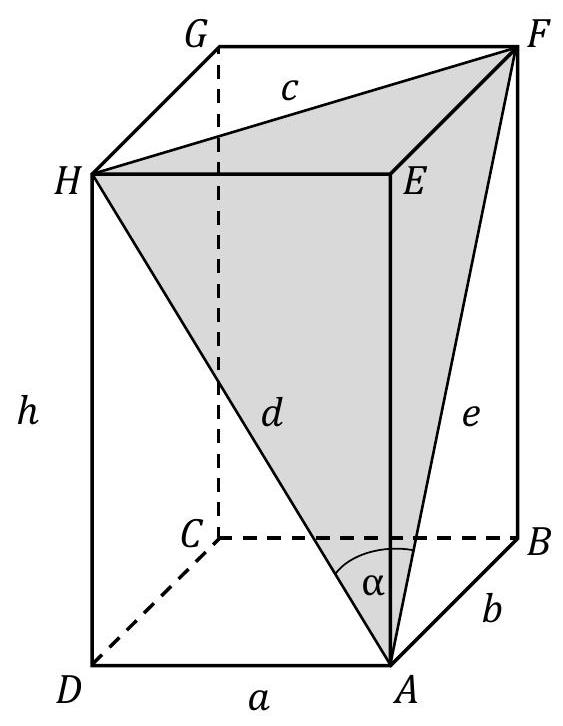
\includegraphics[max width=\textwidth, center]{2025_02_07_368c3175bd12651af85ag-29}

Obliczamy $\cos \alpha: \cos ^{2} \alpha=1-\sin ^{2} \alpha=1-\left(\frac{12}{13}\right)^{2}=\frac{25}{169}$ i kąt $\alpha$ jest ostry, więc $\cos \alpha=\frac{5}{13}$. Zatem

$$
\begin{gathered}
c^{2}=d^{2}+e^{2}-2 \cdot 57,2 \cdot \frac{5}{13} \\
c^{2}=d^{2}+e^{2}-44
\end{gathered}
$$

Stąd, wobec $c^{2}=a^{2}+b^{2}$ oraz $d^{2}=h^{2}+a^{2}$ i $e^{2}=h^{2}+b^{2}$, otrzymujemy

$$
\begin{gathered}
a^{2}+b^{2}=h^{2}+a^{2}+h^{2}+b^{2}-44 \\
h=\sqrt{22}
\end{gathered}
$$

\section*{Zadanie 14. (0-6)}
\begin{center}
\begin{tabular}{|l|l|}
\hline
\multicolumn{2}{|c|}{Wymagania egzaminacyjne 2022} \\
\hline
\multicolumn{1}{|c|}{Wymaganie ogólne} & \multicolumn{1}{c|}{Wymagania szczegółowe} \\
\hline
IV. Użycie i tworzenie strategii. & Zdający: \\
 & P8.3) wyznacza równanie prostej, która jest \\
 & równoległa lub prostopadła do prostej danej \\
 & w postaci kierunkowej i przechodzi przez \\
 & dany punkt; \\
 & P8.6) oblicza odległość dwóch punktów; \\
 & R8.1) oblicza odległość punktu od prostej; \\
 & R8.4) oblicza współrzędne oraz długość \\
 & wektora [...]. \\
\hline
\end{tabular}
\end{center}

\section*{Zasady oceniania}
\section*{Zdający otrzymuje}
gdy:

\begin{itemize}
  \item obliczy odległość punktu $A$ od prostej $y=x-1: d=3 \sqrt{2}$
\end{itemize}

\section*{ALBO}
\begin{itemize}
  \item gdy zapisze współrzędne punktu $B$ lub $C$ w zależności od jednej zmiennej, np. $B=\left(x_{B}, x_{B}-1\right), C=\left(x_{C}, x_{C}-1\right)$,\\
ALBO
  \item zapisze równanie z niewiadomymi $x_{B}, y_{B}, x_{C}, y_{C}$ wynikające $z$ warunków zadania, $n p$.
\end{itemize}

$$
\frac{1}{2} \cdot\left|\left(x_{B}+3\right) \cdot\left(y_{C}-2\right)-\left(y_{B}-2\right) \cdot\left(x_{C}+3\right)\right|=15
$$

LUB

$$
\sqrt{\left(x_{C}+3\right)^{2}+\left(y_{C}-2\right)^{2}}=\sqrt{\left(x_{C}-x_{B}\right)^{2}+\left(y_{C}-y_{B}\right)^{2}}
$$

\section*{Zdający otrzymuje}
gdy:

\begin{itemize}
  \item obliczy odległość $d$ punktu $A$ od prostej $y=x-1$ oraz obliczy długości odcinków $A C$ i $B C:|B C|=5 \sqrt{2}, d=3 \sqrt{2}$\\
ALBO
  \item zapisze równanie z niewiadomymi $x_{B}$ i $x_{C}$, np .
\end{itemize}

$$
\frac{1}{2} \cdot\left|\left(x_{B}+3\right) \cdot\left(x_{C}-3\right)-\left(x_{B}-3\right) \cdot\left(x_{C}+3\right)\right|=15
$$

LUB

$$
\sqrt{\left(x_{C}+3\right)^{2}+\left(x_{C}-3\right)^{2}}=\sqrt{\left(x_{C}-x_{B}\right)^{2}+\left(x_{C}-x_{B}\right)^{2}}
$$

ALBO

\begin{itemize}
  \item wyznaczy równanie prostej $C S$, w którym współczynniki są zależne od $x_{B}$ : $y-\frac{x_{B}+1}{2}=-\frac{x_{B}+3}{x_{B}-3} \cdot\left(x-\frac{x_{B}-3}{2}\right)$ (sposób 3.),
\end{itemize}

ALBO

\begin{itemize}
  \item zapisze układ dwóch równań z czterema niewiadomymi $x_{B}, y_{B}, x_{C}, y_{C}, \mathrm{np}$.\\
$\frac{1}{2} \cdot\left|\left(x_{B}+3\right) \cdot\left(y_{C}-2\right)-\left(y_{B}-2\right) \cdot\left(x_{C}+3\right)\right|=15$\\
i $\sqrt{\left(x_{C}+3\right)^{2}+\left(y_{C}-2\right)^{2}}=\sqrt{\left(x_{C}-x_{B}\right)^{2}+\left(y_{C}-y_{B}\right)^{2}}$.
\end{itemize}

\section*{Zdający otrzymuje}
\begin{itemize}
  \item zapisze równanie, w którym niewiadomymi są wspótrzędne $x_{C}$ oraz $y_{C}$ punktu $C$, np. $\sqrt{\left(x_{C}+3\right)^{2}+\left(y_{C}-2\right)^{2}}=5 \sqrt{2}$\\
ALBO
  \item wyznaczy odległość $A C$ w zależności od pierwszej współrzędnej punktu $C$ : $|A C|=\sqrt{\left(x_{C}-(-3)\right)^{2}+\left(x_{C}-1-2\right)^{2}}$ oraz obliczy odległość $d$ punktu $A$ od prostej $y=x-1: d=3 \sqrt{2}$,\\
ALBO
  \item zapisze układ dwóch równań z dwiema niewiadomymi $x_{B}$ i $x_{C}, \mathrm{np}$.\\
$\frac{1}{2} \cdot\left|\left(x_{B}+3\right) \cdot\left(x_{C}-3\right)-\left(x_{B}-3\right) \cdot\left(x_{C}+3\right)\right|=15$\\
i $\sqrt{\left(x_{C}+3\right)^{2}+\left(x_{C}-3\right)^{2}}=\sqrt{\left(x_{C}-x_{B}\right)^{2}+\left(x_{C}-x_{B}\right)^{2}}$,\\
ALBO
  \item wyznaczy wspórrzędne punktu $C$ w zależności od $x_{B}$ :\\
$C=\left(\frac{x_{B}^{2}-9}{2 x_{B}}, \frac{x_{B}^{2}-2 x_{B}-9}{2 x_{B}}\right)$ (sposób 3.),\\
ALBO
  \item zapisze jedno z równań z dwiema niewiadomymi $x_{B}$ i $y_{B}$ :\\
$\sqrt{\left(x_{B}-0\right)^{2}+\left(y_{B}+1\right)^{2}}=\sqrt{2}$ lub $\sqrt{\left(x_{B}-0\right)^{2}+\left(y_{B}+1\right)^{2}}=9 \sqrt{2}$ (sposób 4.),\\
ALBO
  \item zapisze równanie z dwiema niewiadomymi $x_{C}$ i $y_{C}$ :\\
$\sqrt{\left(x_{C}-0\right)^{2}+\left(y_{C}+1\right)^{2}}=4 \sqrt{2}$ (sposób 4.).
\end{itemize}

\section*{Zdający otrzymuje}
gdy:

\begin{itemize}
  \item zapisze równanie z jedną niewiadomą, pozwalające wyznaczyć współrzędne punktu $C$ lub punktu $B$, np. $\sqrt{\left(x_{C}+3\right)^{2}+\left(x_{C}-3\right)^{2}}=5 \sqrt{2}$\\
LUB
\end{itemize}

$$
\sqrt{\left(4-x_{B}\right)^{2}+\left(4-x_{B}\right)^{2}}=5 \sqrt{2}
$$

LUB

$$
\sqrt{\left(x_{C}-0\right)^{2}+\left(x_{C}-1+1\right)^{2}}=4 \sqrt{2}
$$

ALBO

\begin{itemize}
  \item zapisze równanie z niewiadomą $x_{B}$ :\\
$\left(\left(x_{B}+3\right)^{2}+\left(x_{B}-3\right)^{2}\right)\left(\left(\frac{x_{B}^{2}-9}{2 x_{B}}-\frac{x_{B}-3}{2}\right)^{2}+\left(\frac{x_{B}^{2}-2 x_{B}-9}{2 x_{B}}-\frac{x_{B}+1}{2}\right)^{2}\right)=900$ (sposób 3.),\\
ALBO
  \item zapisze dwa równania z niewiadomą $x_{B}$ :\\
$\sqrt{\left(x_{B}-0\right)^{2}+\left(x_{B}-1+1\right)^{2}}=\sqrt{2}$ i $\sqrt{\left(x_{B}-0\right)^{2}+\left(x_{B}-1+1\right)^{2}}=9 \sqrt{2}$ (sposób 4.).
\end{itemize}

\section*{Zdający otrzymuje}
gdy nie utożsamia żadnego wierzchołka $B$ z żadnym $z$ wierzchołków $C$ (ani $C$ z $B$ ) oraz spełni jeden z poniższych warunków:

\begin{enumerate}
  \item obliczy odcięte punktów $C_{1}$ i $C_{2}$
  \item obliczy odcięte punktów $B_{1}, B_{2}, B_{3}, B_{4}$
  \item obliczy odciętą jednego z punktów $C$ i odcięte odpowiadających temu punktowi dwóch punktów $B$
  \item obliczy odcięte dwóch punktów $B$ i odcięte punktów $C$, odpowiadających tym punktom $B$.
\end{enumerate}

\section*{Zdający otrzymuje}
gdy obliczy współrzędne punktów $B$ i $C$ oraz zapisze te punkty w odpowiednich parach:\\
$C=(4,3)$ i $B=(-1,-2)$ oraz\\
$C=(4,3)$ i $B=(9,8)$, oraz\\
$C=(-4,-5)$ i $B=(1,0)$, oraz\\
$C=(-4,-5)$ i $B=(-9,-10)$.

\section*{Uwagi:}
\begin{enumerate}
  \item Jeśli zdający obliczy długości odcinków $A D, A C$ i $C D$ (punkt $D$ jest rzutem prostokątnym punktu $A$ na prostą o równaniu $y=x-1$ ) i odczyta współrzędne punktu $C$ z rysunku, gubiąc jedno rozwiązanie, to otrzymuje 4 punkty.
  \item Jeśli zdający rozważa trójkąt równoramienny $A B C$, w którym $|A B|=|A C|$, to za całe rozwiązanie może otrzymać co najwyżej 1 punkt (za obliczenie odległości punktu $A$ od prostej $B C$ lub zapisanie współrzędnych punktu $B$ (lub $C$ ) za pomocą jednej zmiennej, lub zapisanie równania $\left.\frac{1}{2} \cdot\left|\left(x_{B}+3\right) \cdot\left(y_{C}-2\right)-\left(y_{B}-2\right) \cdot\left(x_{C}+3\right)\right|=15\right)$, o ile nie nabył praw do innej punktacji.
  \item Jeśli zdający popełni w rozwiązaniu błąd merytoryczny (np. zamiana miejscami wspórrzędnych punktu, błędne zastosowanie wzoru na odległość punktu od prostej, błędne zastosowanie wzorów skróconego mnożenia, stosowanie nieistniejącego wzoru $\sqrt{t+u}=\sqrt{t}+\sqrt{u}$, błędnie zapisana równość wynikająca z twierdzenia Pitagorasa) i konsekwentnie do popełnionego błędu rozwiąże zadanie do końca, to za całe rozwiązanie może otrzymać co najwyżej 4 punkty.
  \item Jeśli zdający popełni w rozwiązaniu błąd rachunkowy, w konsekwencji którego otrzymuje dwie pary punktów, to może otrzymać co najwyżej 5 punktów.
  \item Jeśli zdający narysuje w układzie współrzędnych prostą o równaniu $y=x-1$, zaznaczy punkt $A$ oraz jedną parę punktów $B$ i $C$ i na tej podstawie zapisze współrzędne wierzchołków $B$ i $C$ jednego z trójkątów spełniających warunki zadania oraz sprawdzi rachunkiem, że pole tego trójkąta jest równe 15, to otrzymuje 1 punkt.
\end{enumerate}

\section*{Przykładowe pełne rozwiązania}
Sposób 1.\\
Obliczamy odległość $d$ punktu $A$ od prostej $x-y-1=0: d=\frac{|-3-2-1|}{\sqrt{2}}=3 \sqrt{2}$.\\
Obliczona odległość $d$ jest równa wysokości trójkąta $A B C$ poprowadzonej z wierzchołka $A$ na bok $B C$.\\
Obliczamy długość boku $|B C|$ :

$$
\begin{gathered}
P_{\triangle A B C}=\frac{1}{2} \cdot d \cdot|B C| \\
|B C|=\frac{2 P_{\triangle A B C}}{d}=5 \sqrt{2}
\end{gathered}
$$

Niech $x_{C}$ oznacza pierwszą współrzędną punktu $C$. Punkt $C$ leży na prostej o równaniu $y=x-1$, zatem $C=\left(x_{C}, x_{C}-1\right)$.\\
Korzystając z warunku $|A C|=|B C|$ oraz ze wzoru na długość odcinka, otrzymujemy kolejno

$$
\begin{gathered}
\sqrt{\left(x_{C}-(-3)\right)^{2}+\left(x_{C}-1-2\right)^{2}}=5 \sqrt{2} \\
\sqrt{\left(x_{C}+3\right)^{2}+\left(x_{C}-3\right)^{2}}=5 \sqrt{2} \\
x_{C}^{2}+6 x_{C}+9+x_{C}^{2}-6 x_{C}+9=50 \\
2 x_{C}^{2}-32=0 \\
2\left(x_{C}-4\right)\left(x_{C}+4\right)=0 \\
x_{C}=4 \text { lub } x_{C}=-4
\end{gathered}
$$

Zatem $C=(4,3)$ lub $C=(-4,-5)$.\\
Niech $x_{B}$ oznacza pierwszą wspórłzędną punktu $B$. Punkt $B$ leży na prostej o równaniu $y=x-1$, zatem $B=\left(x_{B}, x_{B}-1\right)$.\\
Ponieważ $|B C|=5 \sqrt{2}$, więc dla $C=(4,3)$ otrzymujemy

$$
\begin{gathered}
\sqrt{\left(4-x_{B}\right)^{2}+\left(3-\left(x_{B}-1\right)\right)^{2}}=5 \sqrt{2} \\
\sqrt{\left(4-x_{B}\right)^{2}+\left(4-x_{B}\right)^{2}}=5 \sqrt{2} \\
2 \cdot\left(4-x_{B}\right)^{2}=50 \\
\left|4-x_{B}\right|=5 \\
x_{B}=-1 \text { lub } x_{B}=9
\end{gathered}
$$

Zatem $B=(-1,-2)$ lub $B=(9,8)$.

Obliczamy współrzędne punktu $B$ dla $C=(-4,-5)$ :

$$
\begin{gathered}
|B C|=5 \sqrt{2} \\
\sqrt{\left(-4-x_{B}\right)^{2}+\left(-5-\left(x_{B}-1\right)\right)^{2}}=5 \sqrt{2} \\
\sqrt{\left(-4-x_{B}\right)^{2}+\left(-4-x_{B}\right)^{2}}=5 \sqrt{2} \\
2 \cdot\left(-4-x_{B}\right)^{2}=50 \\
\left|4+x_{B}\right|=5 \\
x_{B}=1 \text { lub } x_{B}=-9
\end{gathered}
$$

Zatem $B=(1,0)$ lub $B=(-9,-10)$.\\
Warunki zadania spełniają cztery pary punktów:\\
$C=(4,3)$ i $B=(-1,-2)$ oraz\\
$C=(4,3)$ i $B=(9,8)$, oraz\\
$C=(-4,-5)$ i $B=(1,0)$, oraz\\
$C=(-4,-5)$ i $B=(-9,-10)$.

\section*{Uwaga:}
Współrzędne punktu $C$ możemy otrzymać, rozwiązując układ równań\\
$\left\{\begin{array}{l}y=x-1 \\ (x+3)^{2}+(y-2)^{2}=50\end{array}\right.$

Sposób 2.\\
Punkty $B$ i $C$ leżą na prostej o równaniu $y=x-1$, zatem $B=\left(x_{B}, x_{B}-1\right)$ oraz $C=\left(x_{C}, x_{C}-1\right)$.\\
Korzystamy ze wzoru na pole trójkąta

$$
P_{\triangle A B C}=\frac{1}{2} \cdot\left|\left(x_{B}-x_{A}\right)\left(y_{C}-y_{A}\right)-\left(y_{B}-y_{A}\right)\left(x_{C}-x_{A}\right)\right|
$$

i uwzględniamy warunek $P_{\triangle A B C}=15$ :

$$
\begin{gathered}
P_{A B C}=\frac{1}{2} \cdot\left|\left(x_{B}+3\right) \cdot\left(x_{C}-1-2\right)-\left(x_{B}-1-2\right) \cdot\left(x_{C}+3\right)\right| \\
15=\frac{1}{2}\left|6 x_{C}-6 x_{B}\right| \\
5=\left|x_{C}-x_{B}\right|
\end{gathered}
$$

Stąd iz tego, że $|A C|=|B C|$, otrzymujemy układ równań

$$
\left\{\begin{array}{l}
|A C|=|B C| \\
\left|x_{C}-x_{B}\right|=5
\end{array}\right.
$$

Zatem\\
(1) $\left\{\begin{array}{l}\sqrt{\left(x_{C}+3\right)^{2}+\left(x_{C}-3\right)^{2}}=\sqrt{\left(x_{C}-x_{B}\right)^{2}+\left(x_{C}-x_{B}\right)^{2}} \\ x_{C}-x_{B}=5\end{array}\right.$\\
lub\\
(2) $\left\{\begin{array}{l}\sqrt{\left(x_{C}+3\right)^{2}+\left(x_{C}-3\right)^{2}}=\sqrt{\left(x_{C}-x_{B}\right)^{2}+\left(x_{C}-x_{B}\right)^{2}} \\ x_{C}-x_{B}=-5\end{array}\right.$

Rozwiązujemy układ równań (1):

$$
\left\{\begin{array}{l}
x_{C}^{2}+6 x_{C}+9+x_{C}^{2}-6 x_{C}+9=5^{2}+5^{2} \\
x_{C}-x_{B}=5
\end{array}\right.
$$

Z pierwszego równania otrzymujemy równanie kwadratowe $2 x_{C}^{2}+18=50$. Stąd $x_{C}=4$ lub $x_{C}=-4$.\\
Obliczamy współrzędne punktów $B$ i $C$.\\
Dla $x_{C}=4$ otrzymujemy $C=(4,3)$ i $B=(-1,-2)$.\\
Dla $x_{C}=-4$ otrzymujemy $C=(-4,-5)$ i $B=(-9,-10)$.\\
Rozwiązujemy układ równań (2):

$$
\left\{\begin{array}{l}
x_{C}^{2}+6 x_{C}+9+x_{C}^{2}-6 x_{C}+9=5^{2}+5^{2} \\
x_{C}-x_{B}=-5
\end{array}\right.
$$

Z pierwszego równania otrzymujemy równanie kwadratowe $2 x_{C}^{2}+18=50$. Stąd $x_{C}=4$ lub $x_{C}=-4$.\\
Obliczamy współrzędne punktów $B$ i $C$.\\
Dla $x_{C}=4$ otrzymujemy $C=(4,3)$ i $B=(9,8)$.\\
Dla $x_{C}=-4$ otrzymujemy $C=(-4,-5)$ i $B=(1,0)$.\\
Warunki zadania spełniają cztery pary punktów:\\
$C=(4,3)$ i $B=(-1,-2)$ oraz\\
$C=(4,3)$ i $B=(9,8)$, oraz\\
$C=(-4,-5)$ i $B=(1,0)$, oraz\\
$C=(-4,-5)$ i $B=(-9,-10)$.

\section*{Sposób 3.}
Niech $x_{B}$ oznacza pierwszą współrzędną punktu $B$. Punkt $B$ leży na prostej o równaniu $y=x-1$, zatem $B=\left(x_{B}, x_{B}-1\right)$. Środek $S$ podstawy $A B$ ma wspórzzędne

$$
S=\left(\frac{x_{A}+x_{B}}{2}, \frac{y_{A}+y_{B}}{2}\right)=\left(\frac{-3+x_{B}}{2}, \frac{2+x_{B}-1}{2}\right)=\left(\frac{x_{B}-3}{2}, \frac{x_{B}+1}{2}\right)
$$

Jeśli $x_{B}=x_{A}=-3$, to wtedy $S=\left(\frac{-3-3}{2}, \frac{-3+1}{2}\right)=(-3,-1)$, prosta $A B$ ma równanie $x=-3$, więc prosta zawierająca wysokość trójkąta $A B C$ opuszczoną z wierzchołka $C$ ma równanie $y=-1$. Wobec tego $C=\left(x_{C},-1\right)$. Punkt $C$ leży na prostej o równaniu\\
$y=x-1$, więc $-1=x_{C}-1$, czyli $x_{C}=0$. Zatem $C=(0,-1)$. Podstawa $A B$ trójkąta $A B C$ ma wtedy długość $|A B|=6$, a wysokość $S C$ jest równa $|S C|=3$. Pole trójkąta jest wtedy równe

$$
P_{A B C}=\frac{1}{2} \cdot|A B| \cdot|S C|=\frac{1}{2} \cdot 6 \cdot 3=9 \neq 15
$$

Zatem $x_{B} \neq-3$, co oznacza, że prostą $A B$ można opisać równaniem kierunkowym. Współczynnik kierunkowy tej prostej jest równy

$$
a_{A B}=\frac{y_{B}-y_{A}}{x_{B}-x_{A}}=\frac{x_{B}-1-2}{x_{B}-(-3)}=\frac{x_{B}-3}{x_{B}+3}
$$

Jeśli $x_{B}=3$, to wtedy $S=\left(\frac{3-3}{2}, \frac{3+1}{2}\right)=(0,2), y_{B}=2$ i prosta $A B$ ma równanie $y=2$, więc prosta zawierająca wysokość trójkąta $A B C$ opuszczoną z wierzchołka $C$ ma równanie $x=0$. Wobec tego $C=(0,-1)$. Podstawa $A B$ trójkąta $A B C$ ma wtedy długość $|A B|=6$, a wysokość $S C$ jest równa $|S C|=3$. Pole trójkąta jest wtedy równe

$$
P_{A B C}=\frac{1}{2} \cdot|A B| \cdot|S C|=\frac{1}{2} \cdot 6 \cdot 3=9 \neq 15
$$

Zatem $x_{B} \neq 3$.\\
Prosta $S C$ jest prostopadła do prostej $A B$, więc współczynnik kierunkowy prostej $S C$ jest równy

$$
a_{S C}=-\frac{x_{B}+3}{x_{B}-3}
$$

Zatem równanie prostej SC ma postać

$$
\begin{gathered}
y-y_{S}=a_{S C}\left(x-x_{S}\right) \\
y-\frac{x_{B}+1}{2}=-\frac{x_{B}+3}{x_{B}-3} \cdot\left(x-\frac{x_{B}-3}{2}\right) \\
y=-\frac{x_{B}+3}{x_{B}-3} \cdot x+x_{B}+2
\end{gathered}
$$

Wyznaczamy współrzędne punktu $C$, rozwiązując układ równań $\left\{\begin{array}{l}y=x-1 \\ y=-\frac{x_{B}+3}{x_{B}-3} \cdot x+x_{B}+2\end{array}\right.$ Stąd

$$
\begin{gathered}
\left(\frac{x_{B}+3}{x_{B}-3}+1\right) \cdot x=x_{B}+3 \\
\frac{2 x_{B}}{x_{B}-3} \cdot x=x_{B}+3
\end{gathered}
$$

Gdy $x_{B}=0$, to równanie jest sprzeczne, więc $x_{B} \neq 0$. Możemy zatem podzielić obie strony równania przez $\frac{2 x_{B}}{x_{B}-3}$, otrzymując

$$
x=\frac{\left(x_{B}+3\right) \cdot\left(x_{B}-3\right)}{2 x_{B}}=\frac{x_{B}^{2}-9}{2 x_{B}}
$$

Zatem $y=\frac{\left(x_{B}\right)^{2}-9}{2 x_{B}}-1=\frac{\left(x_{B}\right)^{2}-2 x_{B}-9}{2 x_{B}}$, czyli $C=\left(\frac{\left(x_{B}\right)^{2}-9}{2 x_{B}}, \frac{\left(x_{B}\right)^{2}-2 x_{B}-9}{2 x_{B}}\right)$.\\
Pole trójkąta $A B C$ jest równe 15 , więc $\frac{1}{2} \cdot|A B| \cdot|S C|=15$ i stąd otrzymujemy kolejno

$$
\begin{gathered}
|A B|^{2} \cdot|S C|^{2}=900 \\
\left(\left(x_{B}+3\right)^{2}+\left(x_{B}-3\right)^{2}\right)\left(\left(\frac{x_{B}^{2}-9}{2 x_{B}}-\frac{x_{B}-3}{2}\right)^{2}+\left(\frac{x_{B}^{2}-2 x_{B}-9}{2 x_{B}}-\frac{x_{B}+1}{2}\right)^{2}\right)=900 \\
\left(2 x_{B}^{2}+18\right)\left(\left(\frac{x_{B}^{2}-9-x_{B}^{2}+3 x_{B}}{2 x_{B}}\right)^{2}+\left(\frac{x_{B}^{2}-2 x_{B}-9-x_{B}^{2}-x_{B}}{2 x_{B}}\right)^{2}\right)=900 \\
2\left(x_{B}^{2}+9\right)\left(\frac{9}{4}\left(\frac{x_{B}-3}{x_{B}}\right)^{2}+\frac{9}{4}\left(\frac{x_{B}+3}{x_{B}}\right)^{2}\right)=900 \\
\left(x_{B}^{2}+9\right)\left(\left(\frac{x_{B}-3}{x_{B}}\right)^{2}+\left(\frac{x_{B}+3}{x_{B}}\right)^{2}\right)=200 \\
\left(x_{B}^{2}+9\right)\left(\frac{x_{B}^{2}-6 x_{B}+9+x_{B}^{2}+6 x_{B}+9}{x_{B}^{2}}\right)=200 \\
\left(x_{B}^{2}+9\right)\left(\frac{2 x_{B}^{2}+18}{x_{B}^{2}}\right)=200 \\
\frac{2}{x_{B}^{2}}\left(x_{B}^{2}+9\right)^{2}=200 \\
\left(x_{B}^{2}+9\right)^{2}=100 x_{B}^{2} \\
\left(x_{B}^{2}+9\right)^{2}-\left(10 x_{B}\right)^{2}=0 \\
\left(x_{B}^{2}+9-10 x_{B}\right)\left(x_{B}^{2}+9+10 x_{B}\right)=0 \\
\left(x_{B}^{2}-10 x_{B}+9\right)\left(x_{B}^{2}+10 x_{B}+9\right)=0 \\
\left(x_{B}-1\right)\left(x_{B}-9\right)\left(x_{B}+1\right)\left(x_{B}+9\right)=0 \\
x_{B}=1 \text { lub } x_{B}=9 \text { lub } x_{B}=-1 \text { lub } x_{B}=-9
\end{gathered}
$$

Gdy $x_{B}=1$, to $B=(1,0)$ i $C=\left(\frac{1^{2}-9}{2 \cdot 1}, \frac{1^{2}-2 \cdot 1-9}{2 \cdot 1}\right)=(-4,-5)$.\\
Gdy $x_{B}=9$, to $B=(9,8)$ i $C=\left(\frac{9^{2}-9}{2 \cdot 9}, \frac{9^{2}-2 \cdot 9-9}{2 \cdot 9}\right)=(4,3)$.\\
Gdy $x_{B}=-1$, to $B=(-1,-2)$ i $C=\left(\frac{(-1)^{2}-9}{2 \cdot(-1)}, \frac{(-1)^{2}-2 \cdot(-1)-9}{2 \cdot(-1)}\right)=(4,3)$.\\
Gdy $x_{B}=-9$, to $B=(-9,-10)$ i $C=\left(\frac{(-9)^{2}-9}{2 \cdot(-9)}, \frac{(-9)^{2}-2 \cdot(-9)-9}{2 \cdot(-9)}\right)=(-4,-5)$.\\
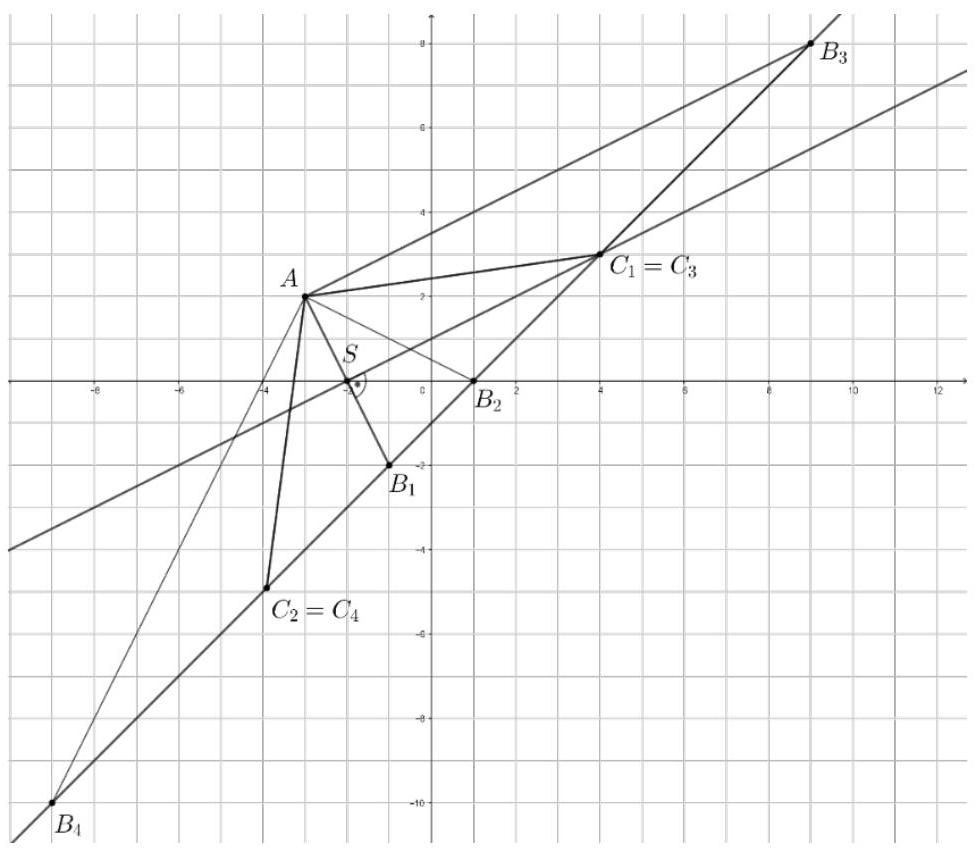
\includegraphics[max width=\textwidth, center]{2025_02_07_368c3175bd12651af85ag-38}

\section*{Sposób 4.}
Obliczamy odległość $d$ punktu $A=(-3,2)$ od prostej $x-y-1=0$ :

$$
d=\frac{|-3-2-1|}{\sqrt{2}}=3 \sqrt{2}
$$

Obliczona odległość jest wysokością trójkąta $A B C$ opuszczoną na prostą $B C$. Ponieważ pole trójkąta $A B C$ jest równe 15 , więc $\frac{1}{2} \cdot d \cdot|B C|=15$ i stąd $|B C|=\frac{30}{3 \sqrt{2}}=5 \sqrt{2}$.\\
Niech $D$ oznacza spodek wysokości trójkąta $A B C$ opuszczonej na prostą $B C$.\\
Obliczamy współrzędne punktu $D$.\\
Prosta prostopadła do prostej o równaniu $y=x-1$, przechodząca przez punkt $A$, jest określona równaniem $y-2=-(x+3)$, czyli $y=-x-1$.\\
Punkt $D$ jest punktem wspólnym prostych $B C$ i $A D$, zatem

$$
x-1=-x-1
$$

więc $x=0$ i $y=0-1=-1$, czyli $D=(0,-1)$.\\
Stosujemy twierdzenie Pitagorasa do trójkąta prostokątnego $A D C$ i wobec\\
$|A D|=d=3 \sqrt{2}$ oraz $|A C|=|B C|=5 \sqrt{2}$ otrzymujemy $|C D|=4 \sqrt{2}$.\\
Niech $C=\left(x_{C}, x_{C}-1\right)$. Ponieważ $|C D|=4 \sqrt{2}$, więc

$$
\sqrt{\left(x_{C}\right)^{2}+\left(x_{C}-1+1\right)^{2}}=4 \sqrt{2}
$$

a stąd

$$
2\left(x_{C}\right)^{2}=32
$$

Zatem $x_{C}{ }^{2}=16$, czyli $x_{C}=4$ lub $x_{C}=-4$.\\
Otrzymujemy punkty o współrzędnych: $C=(4,3)$ lub $C=(-4,-5)$.\\
Należy rozważyć dwa przypadki.\\
Przypadek 1. (gdy punkt $D$ leży na boku $B C$ ).\\
Punkt $B$ leży na prostej o równaniu $y=x-1$, więc $B=\left(x_{B}, x_{B}-1\right)$.

Ponieważ $D$ leży na boku $B C$, więc $|B D|=|B C|-|C D|=5 \sqrt{2}-4 \sqrt{2}=\sqrt{2}$. Zatem

$$
\sqrt{\left(x_{B}-0\right)^{2}+\left(x_{B}-1+1\right)^{2}}=\sqrt{2}
$$

i stąd $2\left(x_{B}\right)^{2}=2$, czyli $x_{B}=1$ lub $x_{B}=-1$.\\
Otrzymujemy punkty o współrzędnych: $B=(1,0)$ lub $B=(-1,-2)$.\\
Gdy $B=(1,0)$, to wtedy $C=(-4,-5)$, a gdy $B=(-1,-2)$, to $C=(4,3)$, gdyż punkt $D$ leży między punktami $B$ i $C$.

Przypadek 2. (gdy punkt $D$ nie leży na boku $B C$ ).\\
Punkt $B$ leży na prostej o równaniu $y=x-1$, więc $B=\left(x_{B}, x_{B}-1\right)$.\\
Ponieważ $D$ nie leży na boku $B C$, więc $|B D|=|C D|+|B C|=4 \sqrt{2}+5 \sqrt{2}=9 \sqrt{2}$. Zatem

$$
\sqrt{\left(x_{B}-0\right)^{2}+\left(x_{B}-1+1\right)^{2}}=9 \sqrt{2}
$$

i stąd $2\left(x_{B}\right)^{2}=81 \cdot 2$, czyli $x_{B}=9$ lub $x_{B}=-9$.\\
Otrzymujemy punkty o wspórrzędnych: $B=(9,8)$ lub $B=(-9,-10)$.\\
Gdy $B=(9,8)$, to wtedy $C=(4,3)$, a gdy $B=(-9,-10)$, to $C=(-4,-5)$, gdyż punkt $B$ leży między punktami $D$ i $C$.

Ostatecznie otrzymujemy cztery trójkąty spełniające warunki zadania o wierzchołkach\\
$A=(-3,2)$ oraz\\
$B=(1,0)$ i $C=(-4,-5)$ lub\\
$B=(-1,-2)$ i $C=(4,3)$, lub\\
$B=(9,8)$ i $C=(4,3)$, lub\\
$B=(-9,-10)$ i $C=(-4,-5)$.

Zadanie 15. (0-7)

\begin{center}
\begin{tabular}{|l|l|}
\hline
\multicolumn{2}{|c|}{Wymagania egzaminacyjne 2022} \\
\hline
\multicolumn{1}{|c|}{Wymaganie ogólne} & \multicolumn{1}{c|}{Wymaganie szczegółowe} \\
\hline
III. Modelowanie matematyczne. & Zdający: \\
 & R11.6) stosuje pochodne do rozwiązywania \\
 & zagadnień optymalizacyjnych. \\
\hline
\end{tabular}
\end{center}

\section*{Zasady oceniania dla sposobu 1.}
\section*{Część a)}
\section*{Zdający otrzymuje}
gdy wyznaczy i zapisze długość a podstawy oraz wysokość $h$ trójkąta w zależności od długości $b$ ramienia trójkąta: $a=18-2 b, h=\sqrt{18 b-81}$.

\section*{Zdający otrzymuje}
gdy zapisze pole trójkąta jako funkcję jednej zmiennej $b$ :

$$
P(b)=\frac{(18-2 b) \cdot \sqrt{18 b-81}}{2}=\frac{\sqrt{(18-2 b)^{2}(18 b-81)}}{2}
$$

\section*{Część b)}
\section*{Zdający otrzymuje}
gdy poprawnie wyznaczy dziedzinę funkcji $P:\left(\frac{9}{2}, 9\right)$.

\section*{Częśćc $\mathbf{c}$}
Zdający otrzymuje ..... 1 pkt\\
gdy wyznaczy wzór pochodnej funkcji $f$, np.

$$
f^{\prime}(b)=(-72+8 b)(18 b-81)+\left(324-72 b+4 b^{2}\right) \cdot 18 \text { lub }
$$

$$
f^{\prime}(b)=216 b^{2}-3240 b+11664, \text { lub } f^{\prime}(b)=216\left(b^{2}-15 b+54\right)
$$

Zdający otrzymuje\\
gdy obliczy miejsca zerowe pochodnej funkcji $f: b=6$.

\section*{Zdający otrzymuje}
gdy zbada znak pochodnej funkcji $f: f^{\prime}(b)>0$ dla $b \in\left(\frac{9}{2}, 6\right)$ oraz $f^{\prime}(b)<0$ dla $b \in(6,9)$ oraz wyznaczy (z uzasadnieniem) wartość zmiennej $b$, dla której funkcja $f$ osiąga wartość największą, np.\\
funkcja $f$ zmiennej $b$ (określona na przedziale $\left(\frac{9}{2}, 9\right)$ ) jest rosnąca w przedziale $\left(\frac{9}{2}, 6\right]$ oraz malejąca w przedziale $[6,9)$, więc w punkcie $b=6$ osiąga największą wartość.

\section*{Zdający otrzymuje}
gdy zapisze, że długość podstawy i ramienia trójkąta o największym polu są równe odpowiednio $a=6$ i $b=6$.

\section*{Uwagi do części c):}
\begin{enumerate}
  \item Badanie znaku pochodnej zdający może opisać w inny sposób, np. szkicując wykres funkcji, która w ten sam sposób jak pochodna zmienia znak i zaznaczając na rysunku, np. znakami „+" i „", znak pochodnej.
  \item Za poprawne uzasadnienie, że rozważana funkcja posiada wartość największą dla wyznaczonej wartości $b$, przy której pochodna się zeruje, można uznać sytuację, gdy zdający:
\end{enumerate}

\begin{itemize}
  \item opisuje (słownie lub graficznie -np. przy użyciu strzałek) monotoniczność funkcji $f$ lub
  \item zapisuje, że dla wyznaczonej wartości $b$ funkcja $f$ ma maksimum lokalne ijest to jednocześnie jej największa wartość.\\
Jeżeli zdający nie przedstawi takiego uzasadnienia, to za część c) może otrzymać co najwyżej 3 punkty.
\end{itemize}

\begin{enumerate}
  \setcounter{enumi}{2}
  \item Jeśli zdający błędnie wyznaczy dziedzinę funkcji $P$ zmiennej $b$, to może otrzymać punkt za dwa ostatnie kroki w części c) tylko wtedy, gdy wyznaczone przez zdającego miejsce zerowe pochodnej należy do części wspólnej wyznaczonej przez zdającego dziedziny i przedziału $\left(\frac{9}{2}, 9\right)$.
  \item Jeśli zdający uzasadnia istnienie największej wartości funkcji pola trójkąta w zbiorze $\mathbb{R}$, to nie otrzymuje punktu za krok trzeci w części c).
  \item Jeśli w części c) zdający bada błędną funkcję, np. $f(b)=\frac{(18-2 b)(18 b-81)}{2}$, to za część c) otrzymuje 0 punktów.
\end{enumerate}

\section*{Zasady oceniania dla sposobu 2.}
\section*{Część a)}
\section*{Zdajacy otrzymuje}
gdy zapisze długość a podstawy w zależności od długości $b$ ramienia trójkąta oraz długości potrzebnych do zastosowania wzoru Herona : $a=18-2 b, p=\frac{2 b+a}{2}$,\\
$p-a=\frac{2 b-a}{2}, p-b=\frac{a}{2}$.

\section*{Zdający otrzymuje}
 gdy zapisze pole trójkąta jako funkcję jednej zmiennej $b$ :$$
P(b)=\frac{(18-2 b) \cdot \sqrt{18 b-81}}{2}=\frac{\sqrt{(18-2 b)^{2}(18 b-81)}}{2}
$$

\section*{Część b)}
\section*{Zdający otrzymuje}
gdy poprawnie wyznaczy dziedzinę funkcji $P:\left(\frac{9}{2}, 9\right)$.

\section*{Częśćc $\mathbf{c}$}
\section*{Zdający otrzymuje}
gdy zapisze zależność między średnią arytmetyczną i średnią geometryczną :

$$
\frac{2 b-9+9-b+9-b}{3} \geq \sqrt[3]{(2 b-9) \cdot(9-b) \cdot(9-b)}
$$

\section*{Zdający otrzymuje}
\section*{Zdajacy otrzymuje}
gdy zapisze, że długość podstawy i ramienia trójkąta o największym polu są równe odpowiednio $a=6, b=6$.

\section*{Przykładowe pełne rozwiązania}
\section*{Sposób 1.}
a)

Przyjmujemy następujące oznaczenia:\\
$a$ - długość podstawy trójkąta,\\
$b$ - długość ramienia trójkąta,\\
$h$ - wysokość trójkąta.\\
Obwód trójkąta jest równy 18 , więc $a+2 b=18$ i stąd $a=18-2 b$.\\
Z geometrycznych warunków zadania wynika, że $a \in(0,+\infty)$ oraz $b \in(0,+\infty)$, więc $18-2 b>0$, zatem $b \in(0,9)$.\\
Korzystając z twierdzenia Pitagorasa i związku $a=18-2 b$, otrzymujemy

$$
\begin{gathered}
h^{2}=b^{2}-\left(\frac{1}{2} a\right)^{2} \\
h^{2}=b^{2}-\left(\frac{1}{2}(18-2 b)\right)^{2} \\
h^{2}=b^{2}-(9-b)^{2} \\
h^{2}=18 b-81 \\
h=\sqrt{18 b-81}
\end{gathered}
$$

Musi zachodzić $18 b-81>0$, więc $b>\frac{81}{18}$. Zatem $b \in\left(\frac{9}{2}, 9\right)$.\\
Pole trójkąta o podstawie $a$ i wysokości $h$ jest równe $P=\frac{a h}{2}$.\\
Zapisujemy pole trójkąta jako funkcję $P$ zmiennej $b$ :

$$
P(b)=\frac{(18-2 b) \cdot \sqrt{18 b-81}}{2} \quad \text { dla } \quad b \in\left(\frac{9}{2}, 9\right)
$$

b)

Z geometrycznych warunków zadania wynika, że $a \in(0,+\infty)$ oraz $b \in(0,+\infty)$, więc $18-2 b>0$, zatem $b \in(0,9)$.\\
Z warunku trójkąta $2 b>a$, czyli $2 b>18-2 b$, więc $b>\frac{9}{2}$. Zatem $b \in\left(\frac{9}{2}, 9\right)$.\\
Dziedziną tej funkcji jest przedział $\left(\frac{9}{2}, 9\right)$.\\
c)

Przekształcamy wzór funkcji $P$ :

$$
P(b)=\frac{(18-2 b) \cdot \sqrt{18 b-81}}{2}=\frac{\sqrt{(18-2 b)^{2}(18 b-81)}}{2}
$$

Tworzymy funkcję pomocniczą $f$ określoną wzorem\\
$f(b)=(18-2 b)^{2}(18 b-81)$ dla $b \in\left(\frac{9}{2}, 9\right)$.\\
Wyznaczamy pochodną funkcji $f$ :

$$
f^{\prime}(b)=(-72+8 b)(18 b-81)+\left(324-72 b+4 b^{2}\right) \cdot 18=216 b^{2}-3240 b+11664
$$

Obliczamy miejsce zerowe pochodnej funkcji $f$ :

$$
\begin{gathered}
f^{\prime}(b)=0 \\
216 b^{2}-3240 b+11664=0 \quad \text { i } \quad b \in\left(\frac{9}{2}, 9\right) \\
b^{2}-15 b+54=0 \quad \text { i } \quad b \in\left(\frac{9}{2}, 9\right) \\
b=6
\end{gathered}
$$

Ponieważ $f^{\prime}(b)>0$ dla $b \in\left(\frac{9}{2}, 6\right)$ oraz $f^{\prime}(b)<0$ dla $b \in(6,9)$, więc funkcja $f$ jest rosnąca w przedziale $\left(\frac{9}{2}, 6\right\rangle$ oraz malejąca w przedziale $\langle 6,9)$. Zatem funkcja $f$ osiąga wartość największą dla $b=6$.\\
Ponieważ funkcja $g(x)=\sqrt{x}$, określona dla każdej liczby $x \geq 0$, jest funkcją rosnąca, więc funkcja pola $P$ osiąga wartość największą dla tego argumentu, dla którego funkcja $f$ osiąga wartość największą, tj. dla $b=6$. Wtedy $a=18-2 \cdot 6=6$.\\
Spośród rozważanych trójkątów największe pole ma trójkąt równoboczny o boku 6 .

\section*{Sposób 2.}
a)

Przyjmujemy następujące oznaczenia:\\
$a$ - długość podstawy trójkąta,\\
$b$ - długość ramienia trójkąta,\\
$h$ - wysokość trójkąta.\\
Obwód trójkąta jest równy 18 , więc $a+2 b=18$ i stąd $a=18-2 b$.\\
Wyznaczamy pole trójkąta, korzystając ze wzoru Herona.\\
Trójkąt jest równoramienny, więc połowa $p$ obwodu trójkąta jest równa $p=\frac{2 b+a}{2}$ oraz $p-a=\frac{2 b+a}{2}-a=\frac{2 b-a}{2}$ i $p-b=\frac{2 b+a}{2}-b=\frac{a}{2}$.

Zatem

$$
P=\sqrt{\frac{2 b+a}{2} \cdot \frac{2 b-a}{2} \cdot \frac{a}{2} \cdot \frac{a}{2}}
$$

Ponieważ $a=18-2 b>0$, więc

$$
\begin{gathered}
P(b)=\sqrt{\frac{2 b+18-2 b}{2} \cdot \frac{2 b-18+2 b}{2} \cdot \frac{18-2 b}{2} \cdot \frac{18-2 b}{2}} \\
P(b)=\sqrt{9 \cdot(2 b-9) \cdot\left(\frac{18-2 b}{2}\right)^{2}} \\
P(b)=\frac{(18-2 b) \cdot \sqrt{18 b-81}}{2}
\end{gathered}
$$

b)

Wyznaczamy dziedzinę funkcji $P$.\\
Z geometrycznych warunków zadania wynika, że $a \in(0,+\infty)$ oraz $b \in(0,+\infty)$, więc $18-2 b>0$, zatem $b \in(0,9)$.\\
Ponadto $z$ warunku dla trójkąta $2 b>a$, więc $2 b>18-2 b$ i stąd $b>\frac{9}{2}$.\\
Dziedziną funkcji $P$ jest przedział $\left(\frac{9}{2}, 9\right)$.\\
c)

Z nierówności między średnimi arytmetyczną i geometryczną dla liczb dodatnich $2 b-9$, $9-b, 9-b$ otrzymujemy

$$
\begin{gathered}
\frac{2 b-9+9-b+9-b}{3} \geq \sqrt[3]{(2 b-9) \cdot(9-b) \cdot(9-b)} \\
3 \geq \sqrt[3]{(2 b-9) \cdot(9-b)^{2}} \\
27 \geq(2 b-9) \cdot(9-b)^{2}
\end{gathered}
$$

Zatem

$$
\sqrt{(2 b-9) \cdot(9-b)^{2}} \leq 3 \sqrt{3}
$$

przy czym równość zachodzi tylko wtedy, gdy $2 b-9=9-b$, tj. dla $b=6$. Ponieważ

$$
P(b)=\frac{(18-2 b) \cdot \sqrt{18 b-81}}{2}=3 \sqrt{(9-b)^{2} \cdot(2 b-9)}
$$

więc $P(b) \leq 3 \cdot 3 \sqrt{3}$, przy czym równość zachodzi tylko wtedy, gdy $b=6$.\\
Zatem funkcja $P$ osiąga wartość największą dla $b=6$. Wtedy $a=18-2 \cdot 6=6$.

Spośród rozważanych trójkątów największe pole ma trójkąt równoboczny o boku 6.


\end{document}